\documentclass[]{article}
\usepackage{lmodern}
\usepackage{amssymb,amsmath}
\usepackage{ifxetex,ifluatex}
\usepackage{fixltx2e} % provides \textsubscript
\ifnum 0\ifxetex 1\fi\ifluatex 1\fi=0 % if pdftex
  \usepackage[T1]{fontenc}
  \usepackage[utf8]{inputenc}
\else % if luatex or xelatex
  \ifxetex
    \usepackage{mathspec}
  \else
    \usepackage{fontspec}
  \fi
  \defaultfontfeatures{Ligatures=TeX,Scale=MatchLowercase}
\fi
% use upquote if available, for straight quotes in verbatim environments
\IfFileExists{upquote.sty}{\usepackage{upquote}}{}
% use microtype if available
\IfFileExists{microtype.sty}{%
\usepackage{microtype}
\UseMicrotypeSet[protrusion]{basicmath} % disable protrusion for tt fonts
}{}
\usepackage[margin=1in]{geometry}
\usepackage{hyperref}
\hypersetup{unicode=true,
            pdftitle={Melbourne Housing Data Analysis},
            pdfauthor={Subhankar Ghosh},
            pdfborder={0 0 0},
            breaklinks=true}
\urlstyle{same}  % don't use monospace font for urls
\usepackage{color}
\usepackage{fancyvrb}
\newcommand{\VerbBar}{|}
\newcommand{\VERB}{\Verb[commandchars=\\\{\}]}
\DefineVerbatimEnvironment{Highlighting}{Verbatim}{commandchars=\\\{\}}
% Add ',fontsize=\small' for more characters per line
\usepackage{framed}
\definecolor{shadecolor}{RGB}{248,248,248}
\newenvironment{Shaded}{\begin{snugshade}}{\end{snugshade}}
\newcommand{\KeywordTok}[1]{\textcolor[rgb]{0.13,0.29,0.53}{\textbf{#1}}}
\newcommand{\DataTypeTok}[1]{\textcolor[rgb]{0.13,0.29,0.53}{#1}}
\newcommand{\DecValTok}[1]{\textcolor[rgb]{0.00,0.00,0.81}{#1}}
\newcommand{\BaseNTok}[1]{\textcolor[rgb]{0.00,0.00,0.81}{#1}}
\newcommand{\FloatTok}[1]{\textcolor[rgb]{0.00,0.00,0.81}{#1}}
\newcommand{\ConstantTok}[1]{\textcolor[rgb]{0.00,0.00,0.00}{#1}}
\newcommand{\CharTok}[1]{\textcolor[rgb]{0.31,0.60,0.02}{#1}}
\newcommand{\SpecialCharTok}[1]{\textcolor[rgb]{0.00,0.00,0.00}{#1}}
\newcommand{\StringTok}[1]{\textcolor[rgb]{0.31,0.60,0.02}{#1}}
\newcommand{\VerbatimStringTok}[1]{\textcolor[rgb]{0.31,0.60,0.02}{#1}}
\newcommand{\SpecialStringTok}[1]{\textcolor[rgb]{0.31,0.60,0.02}{#1}}
\newcommand{\ImportTok}[1]{#1}
\newcommand{\CommentTok}[1]{\textcolor[rgb]{0.56,0.35,0.01}{\textit{#1}}}
\newcommand{\DocumentationTok}[1]{\textcolor[rgb]{0.56,0.35,0.01}{\textbf{\textit{#1}}}}
\newcommand{\AnnotationTok}[1]{\textcolor[rgb]{0.56,0.35,0.01}{\textbf{\textit{#1}}}}
\newcommand{\CommentVarTok}[1]{\textcolor[rgb]{0.56,0.35,0.01}{\textbf{\textit{#1}}}}
\newcommand{\OtherTok}[1]{\textcolor[rgb]{0.56,0.35,0.01}{#1}}
\newcommand{\FunctionTok}[1]{\textcolor[rgb]{0.00,0.00,0.00}{#1}}
\newcommand{\VariableTok}[1]{\textcolor[rgb]{0.00,0.00,0.00}{#1}}
\newcommand{\ControlFlowTok}[1]{\textcolor[rgb]{0.13,0.29,0.53}{\textbf{#1}}}
\newcommand{\OperatorTok}[1]{\textcolor[rgb]{0.81,0.36,0.00}{\textbf{#1}}}
\newcommand{\BuiltInTok}[1]{#1}
\newcommand{\ExtensionTok}[1]{#1}
\newcommand{\PreprocessorTok}[1]{\textcolor[rgb]{0.56,0.35,0.01}{\textit{#1}}}
\newcommand{\AttributeTok}[1]{\textcolor[rgb]{0.77,0.63,0.00}{#1}}
\newcommand{\RegionMarkerTok}[1]{#1}
\newcommand{\InformationTok}[1]{\textcolor[rgb]{0.56,0.35,0.01}{\textbf{\textit{#1}}}}
\newcommand{\WarningTok}[1]{\textcolor[rgb]{0.56,0.35,0.01}{\textbf{\textit{#1}}}}
\newcommand{\AlertTok}[1]{\textcolor[rgb]{0.94,0.16,0.16}{#1}}
\newcommand{\ErrorTok}[1]{\textcolor[rgb]{0.64,0.00,0.00}{\textbf{#1}}}
\newcommand{\NormalTok}[1]{#1}
\usepackage{longtable,booktabs}
\usepackage{graphicx,grffile}
\makeatletter
\def\maxwidth{\ifdim\Gin@nat@width>\linewidth\linewidth\else\Gin@nat@width\fi}
\def\maxheight{\ifdim\Gin@nat@height>\textheight\textheight\else\Gin@nat@height\fi}
\makeatother
% Scale images if necessary, so that they will not overflow the page
% margins by default, and it is still possible to overwrite the defaults
% using explicit options in \includegraphics[width, height, ...]{}
\setkeys{Gin}{width=\maxwidth,height=\maxheight,keepaspectratio}
\IfFileExists{parskip.sty}{%
\usepackage{parskip}
}{% else
\setlength{\parindent}{0pt}
\setlength{\parskip}{6pt plus 2pt minus 1pt}
}
\setlength{\emergencystretch}{3em}  % prevent overfull lines
\providecommand{\tightlist}{%
  \setlength{\itemsep}{0pt}\setlength{\parskip}{0pt}}
\setcounter{secnumdepth}{0}
% Redefines (sub)paragraphs to behave more like sections
\ifx\paragraph\undefined\else
\let\oldparagraph\paragraph
\renewcommand{\paragraph}[1]{\oldparagraph{#1}\mbox{}}
\fi
\ifx\subparagraph\undefined\else
\let\oldsubparagraph\subparagraph
\renewcommand{\subparagraph}[1]{\oldsubparagraph{#1}\mbox{}}
\fi

%%% Use protect on footnotes to avoid problems with footnotes in titles
\let\rmarkdownfootnote\footnote%
\def\footnote{\protect\rmarkdownfootnote}

%%% Change title format to be more compact
\usepackage{titling}

% Create subtitle command for use in maketitle
\newcommand{\subtitle}[1]{
  \posttitle{
    \begin{center}\large#1\end{center}
    }
}

\setlength{\droptitle}{-2em}
  \title{Melbourne Housing Data Analysis}
  \pretitle{\vspace{\droptitle}\centering\huge}
  \posttitle{\par}
  \author{Subhankar Ghosh}
  \preauthor{\centering\large\emph}
  \postauthor{\par}
  \date{}
  \predate{}\postdate{}

\usepackage{float}
\floatplacement{figure}{H}

\begin{document}
\maketitle

\section{1. Data Processing and
Analysis}\label{data-processing-and-analysis}

In this module I will be following a few steps as I am jotting them
down:

\begin{itemize}
\item
  Since the goal of this analysis is to predict the Price variable,
  hence any missing value of this variable can be discarded from the
  data
\item
  Summarize each variable in the data set and provide simple descriptive
  statistics using tables/plots
\item
  Any important transformations will be shown and explained
\end{itemize}

There are total 34857 observations and 21 variables including the
variable Price.

\textbf{Handling missing values in Price:} We found 7610 observations
with missing Price and we removed them because that is the response
variable so there is no point in trying to impute that. So now we will
deal with only 27247 observations.

\emph{Note:} For categorical variables we replace `\#N/A' values by NA.

I have found broadly 3 categories of features - \textbf{Location based},
\textbf{House related}, \textbf{Seller related.}

\paragraph{Location Based Features}\label{location-based-features}

In this category I have included the features which say anything about
the location of the property. These features are: \textbf{Suburbs,
Address, Postcode, CouncilArea, Lattitude, Longitude, Regionname,
Propertycount.}

\textbf{Address}

The variable \textbf{Address} is unique to each row and therefore
doesnot add any value to the regression process. Since it is a
categorical variable with the number of categories equal to the number
of training examples it does not even make sense to do a one-hot
encoding because then it will just make a diagonal matrix of this
variable. So we will remove Address also.

\textbf{Lattitude and Longitude}

From Figure 1 of Lattitude and Longitude with Price we can see that
there is very minimal variation in Price. We do not see any pattern from
the plot that can help in our regression task of predicting Price.

Along with this variable we have \emph{Suburbs}, \emph{Region Name},
\emph{Council Area} to give us the same location information. So
\textbf{Lattitude} and \textbf{Longitude} variables are redundant and
without much impact in the regression task. We will need to check the
effects of these two variables in regression.

\textbf{Suburbs, Regionname, CouncilArea and PostCode}

If we understand the way land is divided in Melbourne it would be of
much help to us to decide which features should we keep and which ones
we can discard. Well the Melbourne follows a hierarcical land division
strategy.

\begin{figure}
\centering
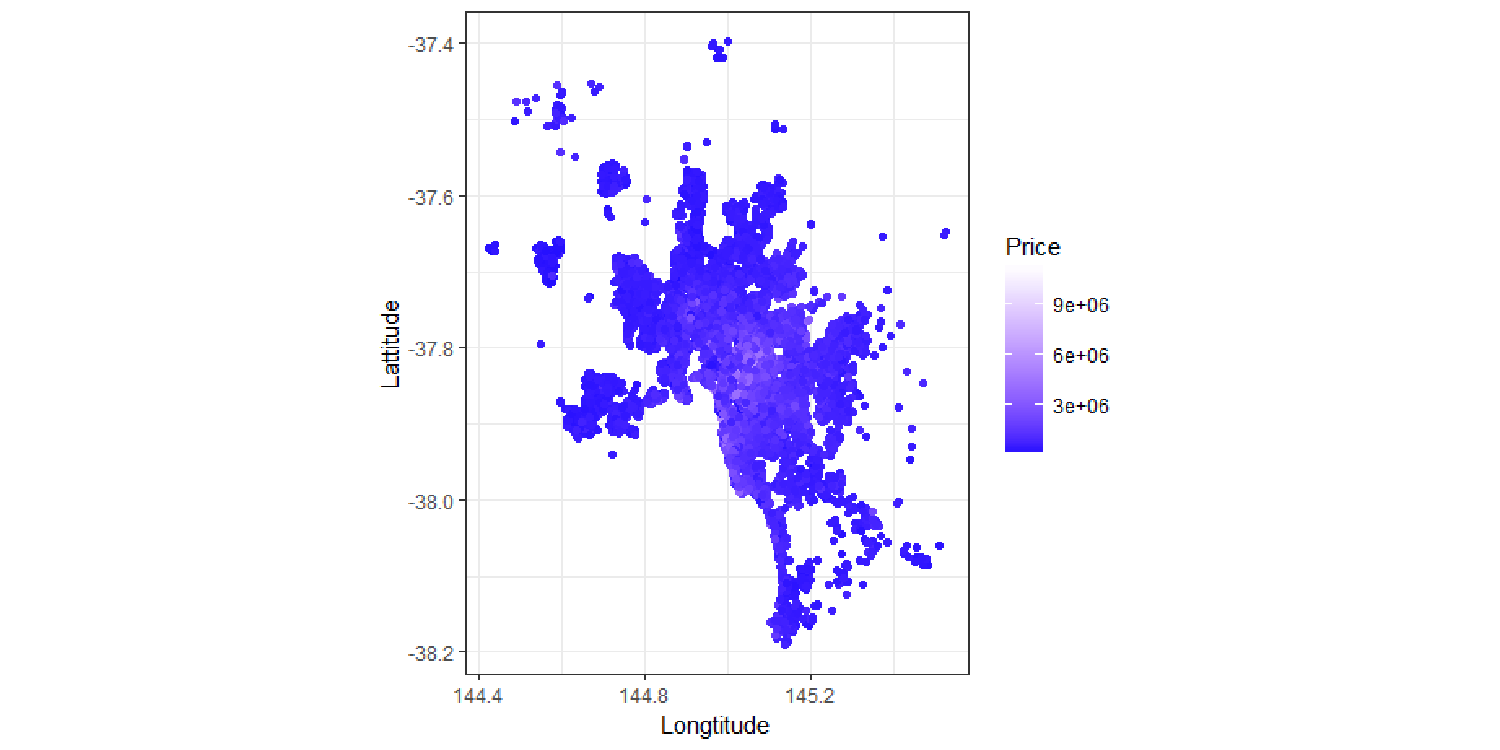
\includegraphics{Report_files/figure-latex/unnamed-chunk-2-1.pdf}
\caption{Lattitude-Longitude with Price}
\end{figure}

The entire area is divided into many Regions \textbf{(Regionname)}. Each
Region in turn is divided into some Council areas \textbf{(CouncilArea)}
and finally each Council area is divided into \textbf{Suburbs.} Every
Suburb is associated with a particular Postal Code \textbf{(Postcode).}

Since every Suburb is associated with a Postcode we can remove the
\textbf{Postcode} as it has a one-to-one relation with Suburb and we do
not want two linearly dependent variables in our regression setup.

\textbf{Regionname:} There are 3 missing values still existing in
Regionname. Looking at these three records we can see that for these
three records other features such as BuildingArea, YearBuilt,
CouncilArea, Regionname, Propertycount, Bedroom2, Bathroom, Car,
Landsize are also NA. Therefore we will remove these three rows.

From the below Figure 2 of Region Name and Price we see that Southern
Metropolitan is the highest followed closely by South Eastern
Metropolitan.

There is not a significant difference between the means of Prices in
each Region but the outliers in Southern Metropolitan make it the
poshest region. We see North Victoria, East Victoria and Western
Victoria distribution to be limited to a close price range while the
highs and lows of other regions are quite far apart.A bimodal
distribution is visible in Western Metropolitan and Eastern Metropolitan
that might suggest a particular type of houses sold more than other
types.

\begin{figure}
\centering
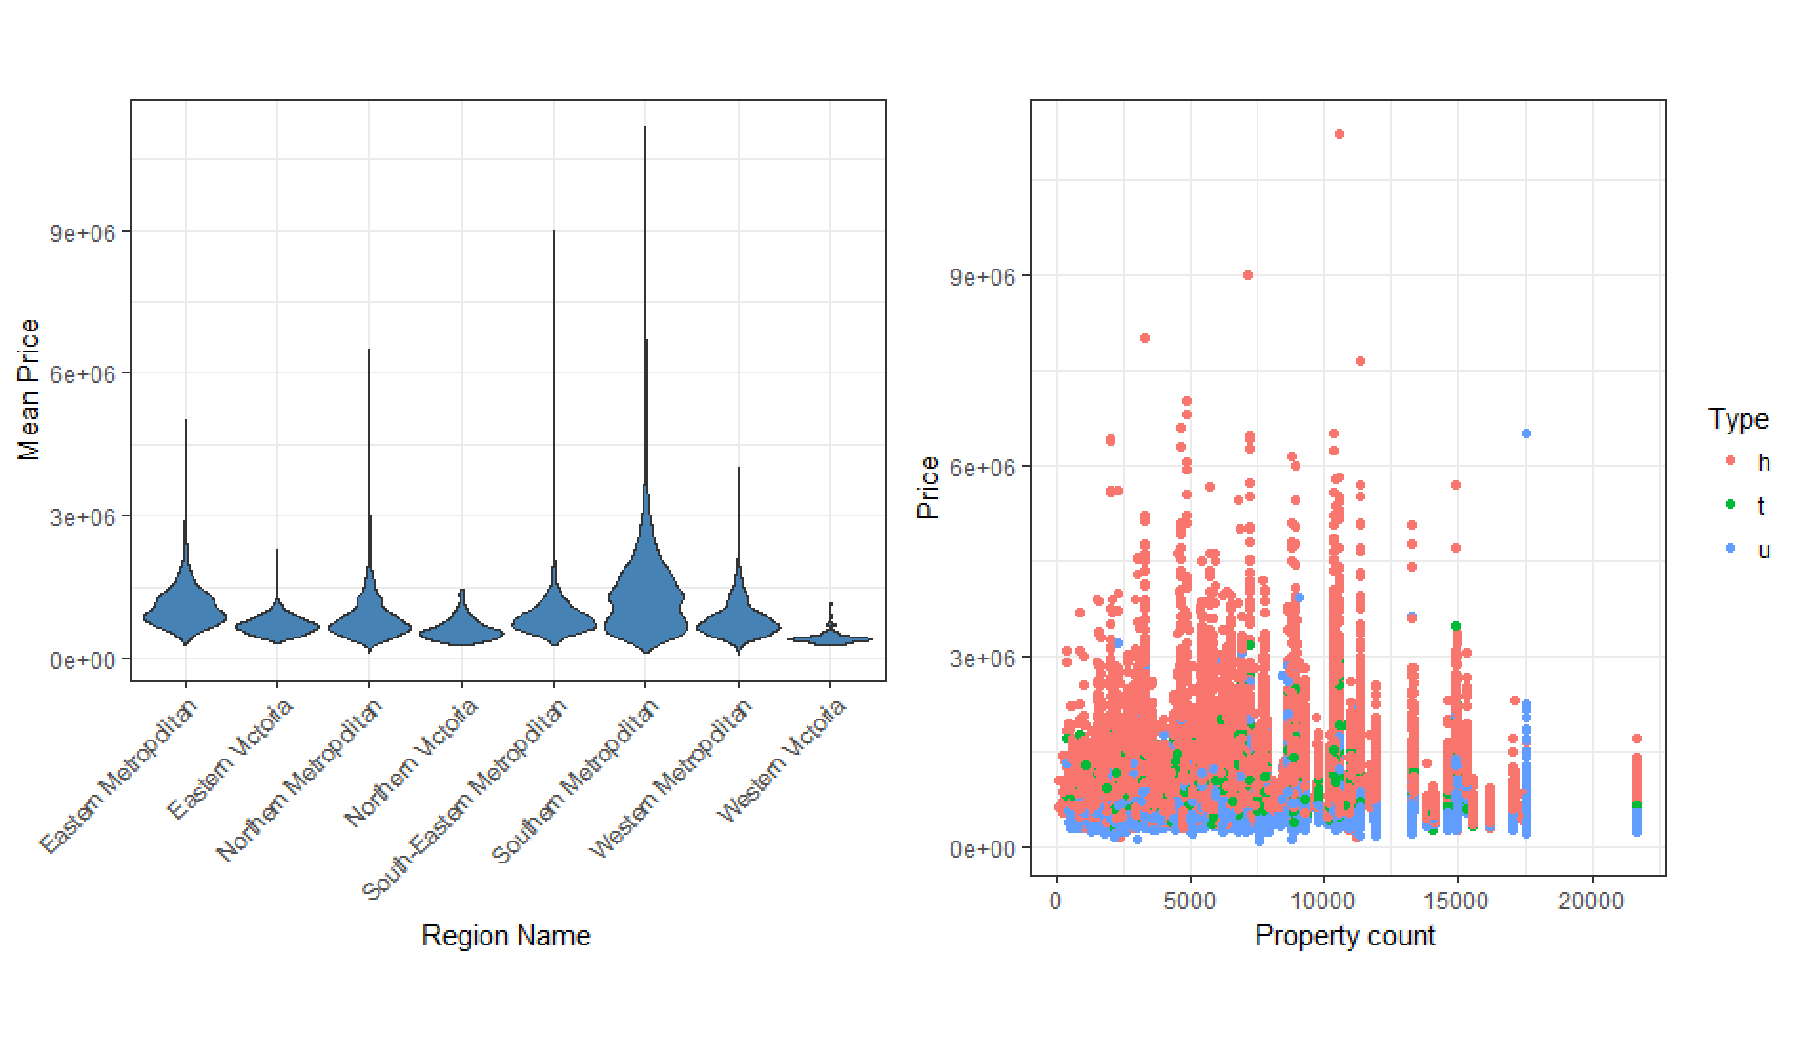
\includegraphics{Report_files/figure-latex/unnamed-chunk-3-1.pdf}
\caption{(a) Region Name with Price (b) Property and Type with Price}
\end{figure}

\textbf{Suburb:} There are 345 Suburbs mentioned in the dataset with
\emph{Reservoir} appearing highest number of times \((727)\) times
followed by \emph{Bentleigh East} \(493\) times. Suburb being a
categorical variable needs to be one-hot encoded to be used in
Regression which might lead us to the problem of the \emph{Curse of
Dimensionality.} So I am keeping it for now but later we might have to
remove it.

\textbf{Property Count and Type:} Property count tells us the number of
houses in each Suburb and Type tells us the type of the property.
\emph{Type} has 3 values:

\begin{itemize}
\tightlist
\item
  h = House, cottage, villa. This category has the costliest properties,
  and it makes sense because an entire house should be more costly than
  an apartment.
\item
  u = Unit, Duplex. This as expected has the lowest values of Price as
  seen in the plot except some exceptions which may be the Units in high
  rise buildings at some prime location of Melbourne.
\item
  t = Townhouse. These are less in number as seen in the plot also they
  come in the medium level range.
\end{itemize}

But we cannot see any pattern or strong relationship with Propertycount
from the Figure 3.

\paragraph{House Related Features}\label{house-related-features}

\textbf{Rooms, Bedroom2} Rooms and Bedroom2 are highly correlated
features with a correlation of \(0.9587\), So we would drop one of them
since we do not want linearly dependent variables. Since Bedroom2 has
6438 missing values so we drop Bedroom2.

\textbf{Landsize and Distance:} Landsize variable has outliers. Its
\(3^{rd} quantile\) value is 664 but its maximum value is 433014, so to
solve this issue we log transform landsize. From the Figure 4(b) of
Distance and log(Landsize) we see that the properties with high prices
mainly lie in the low distance from the \emph{City Center} region mostly
within 20 Km range. Landsize was a surprise since we do not see high
prices for properties with high landsize,they are in the middle range of
landsize that gets the high prices. So high priced properties are those
middle range area-wise and close to the City Center. Also Landsize has
9262 missing values we will impute them with median value.

\begin{figure}
\centering
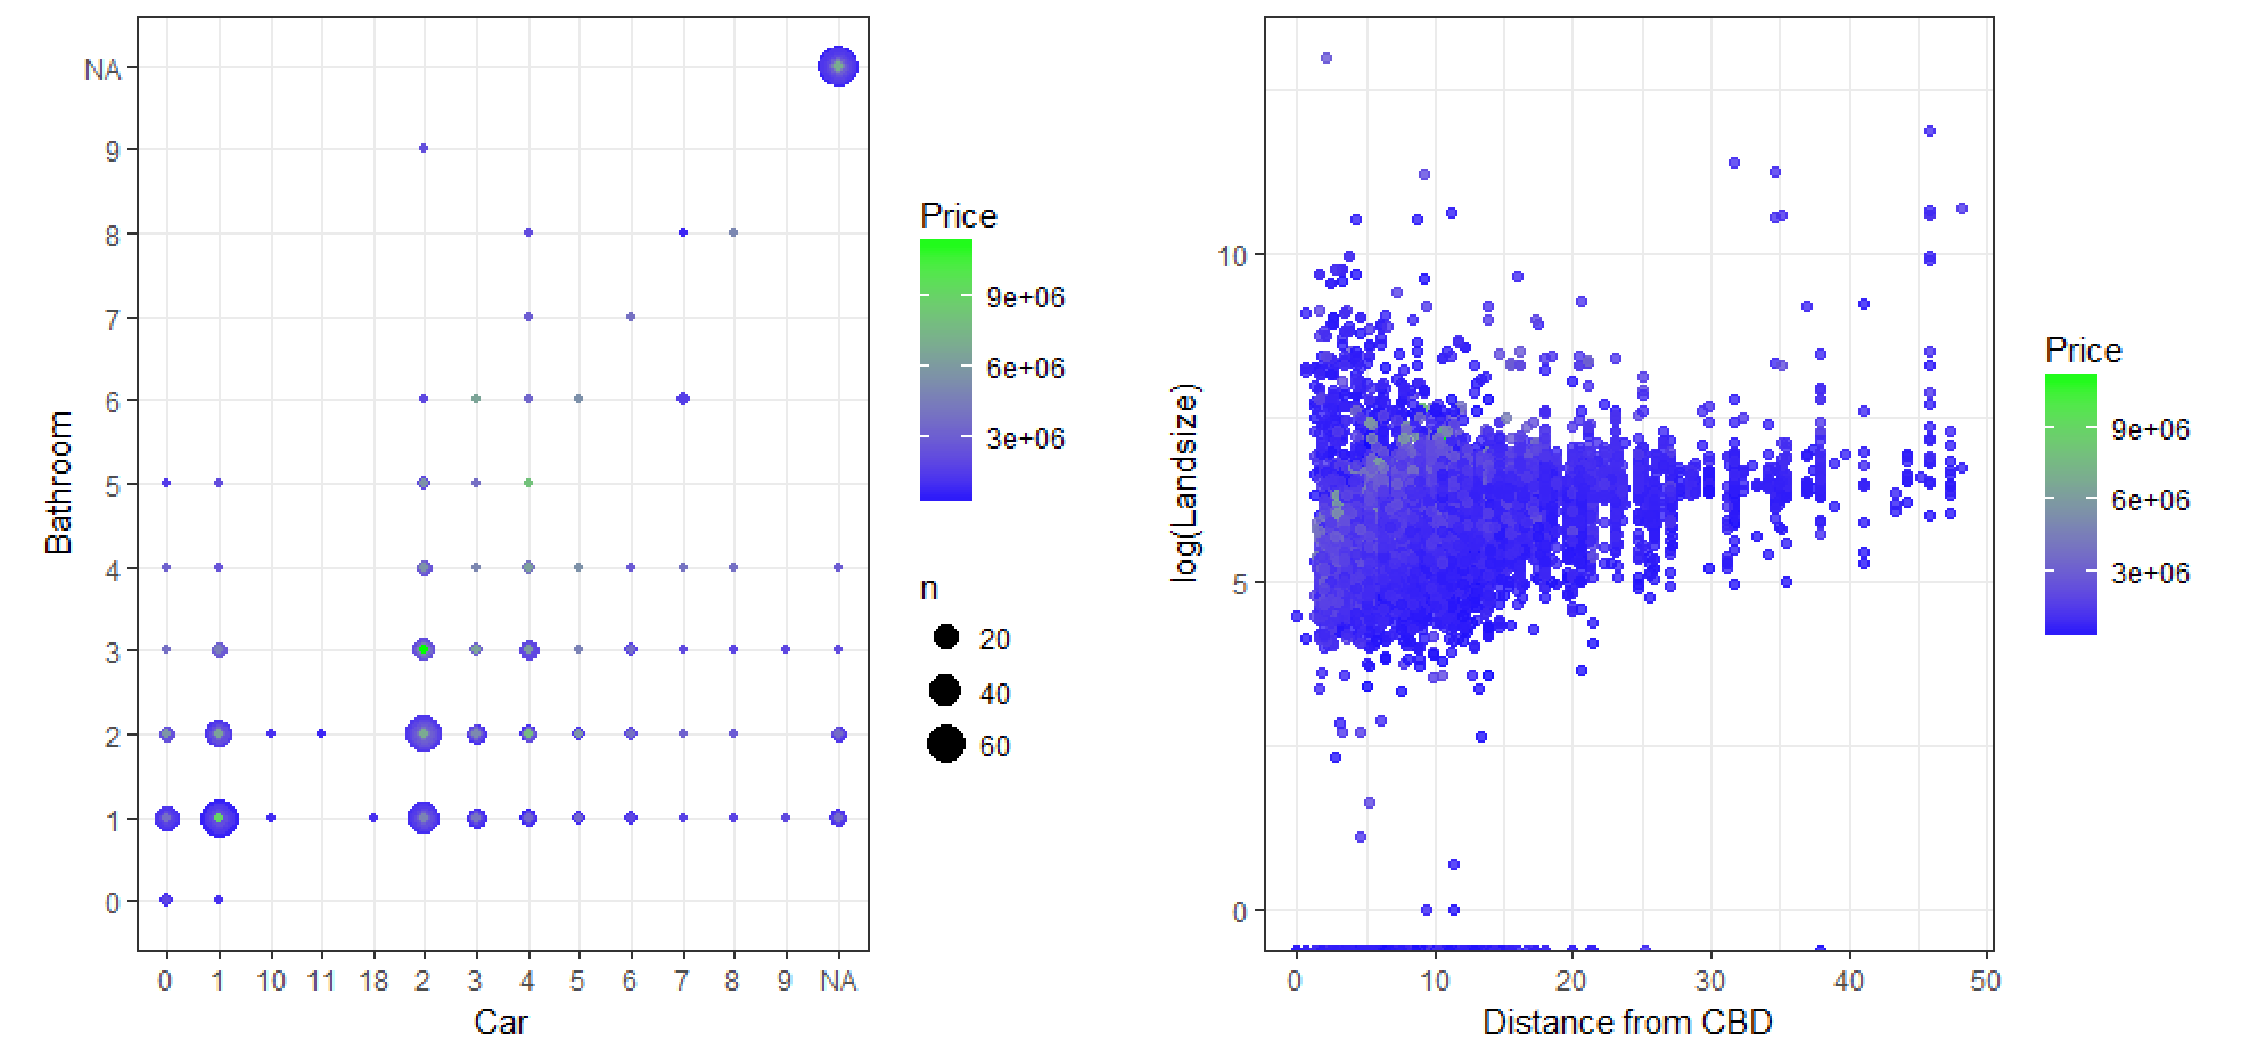
\includegraphics{Report_files/figure-latex/unnamed-chunk-4-1.pdf}
\caption{(a) Bathroom vs Car spots. (b) Landsize vs distance from CBD.}
\end{figure}

\textbf{Bathroom and Car:} Two pretty important features for predicting
price of a property. We expect that more the number of Bathrooms more
will be the price, but the Figure 4(a) shows that is not the case.
Infact there are many high price properties with just one bathroom and
one car. These properties must be the studio apartments or the small
private villas. It would be interesting to look at the kind of property
that have 5 bathrooms and 4 car spots because they consist of only high
priced property.

\textbf{BuildingArea and YearBuilt:} BuildingArea and YearBuilt have
16588 and 15160 missing values which are more than \(50\) percent of the
dataset, so if we impute these missing values with a particular value
then we will be introducing a huge bias to our dataset. That is why we
will remove these columns.

\paragraph{Seller Related Features}\label{seller-related-features}

\textbf{SellerG:} This is a factor variable telling us about the
seller's identity/name. It has 349 unique values, just like Suburb
variable this variable with a lot of categories I do not think will be
very helpful in regression so there is a possibility that we might have
to remove it before applying regression.

\textbf{Method:} Although the means of the properties sold by each of
the method does not differ much as we can see but it is interesting to
see the extreme values of Price we observe in \emph{VB: Vendor Bid} and
\emph{Pl: Property passed in}. For PI Many prospective buyers might
increase their offering from what was bid at auction in order to secure
the property when they realize that it was not sold on auction day
bidding (Meaning of Passed in). VB properties must have been bid at
astronomical prices so that no one can bid higher. \emph{SA: Sold after
auction} some of these cases turn negative as well leading to low
prices.

\begin{figure}
\centering
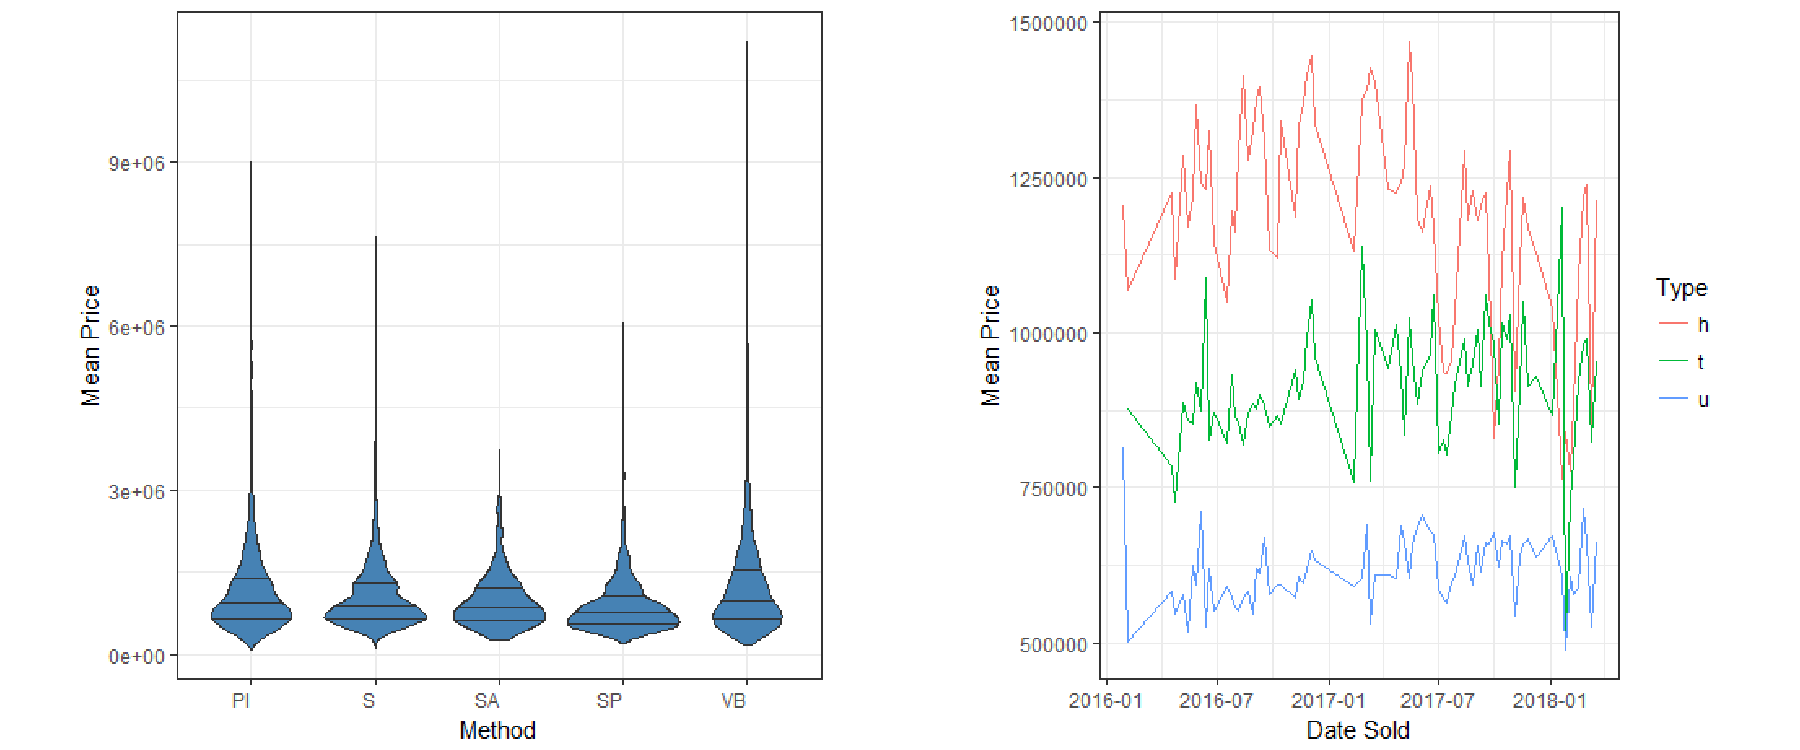
\includegraphics{Report_files/figure-latex/unnamed-chunk-5-1.pdf}
\caption{(a) Price vs Method distribution (b) Price as seen over time}
\end{figure}

\textbf{Date:} Also seems to be an important feature as we see from the
Figure 5(b) that there are many unexpeced ups and downs in the prices in
the late 2018 especially of townhouse and villa properties. The
townhouse prices plummet below the unit properties in early 2018 just
after a boom in their prices. At a similar timeperiod Villa prices drop
quite low compared to their prices.

\begin{figure}
\centering
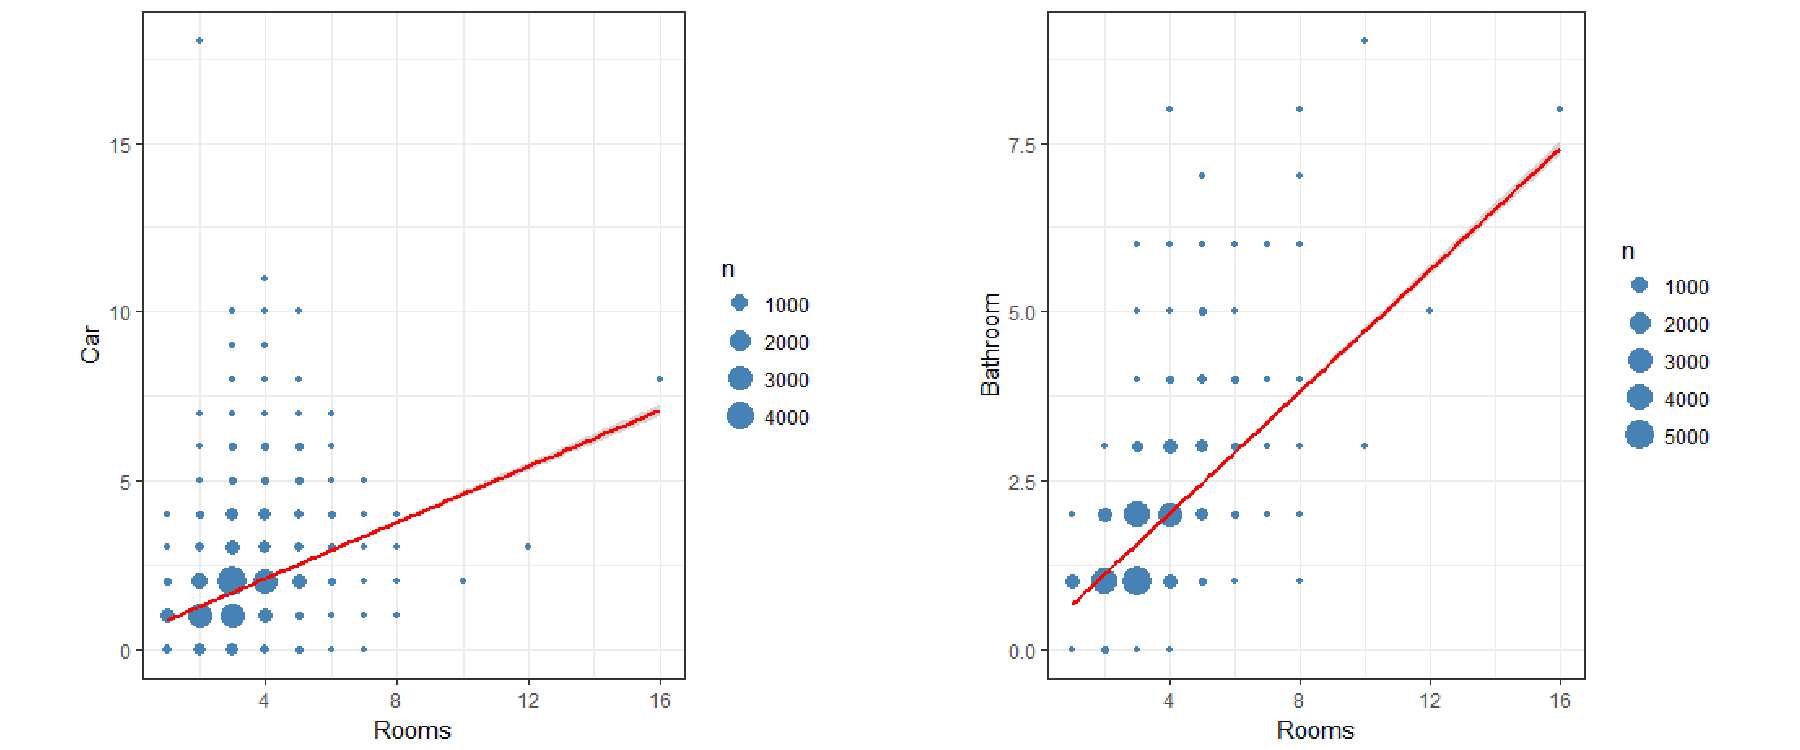
\includegraphics{Report_files/figure-latex/unnamed-chunk-6-1.pdf}
\caption{(a) Car vs Rooms (b) Bathroom vs Rooms}
\end{figure}

\textbf{Dealing with missing values in Bathroom and Cars:} From above
plots we see a clear relationship between Rooms and Car or bathroom. So
we predict the missing values of Car and Bathroom using a linear model
with just Rooms as the predictor.

\pagebreak

\section{2. Cluster Analysis}\label{cluster-analysis}

In this analysis I am planning to use K-means clustering algorithm. We
have some really interesting numerical variables as well as some ordinal
variables which we can convert to numerical variables. For K-means
algorithm we need to decide the number of clusters before hand. Let us
look at the \textbf{distribution of Price.}

\begin{figure}
\centering
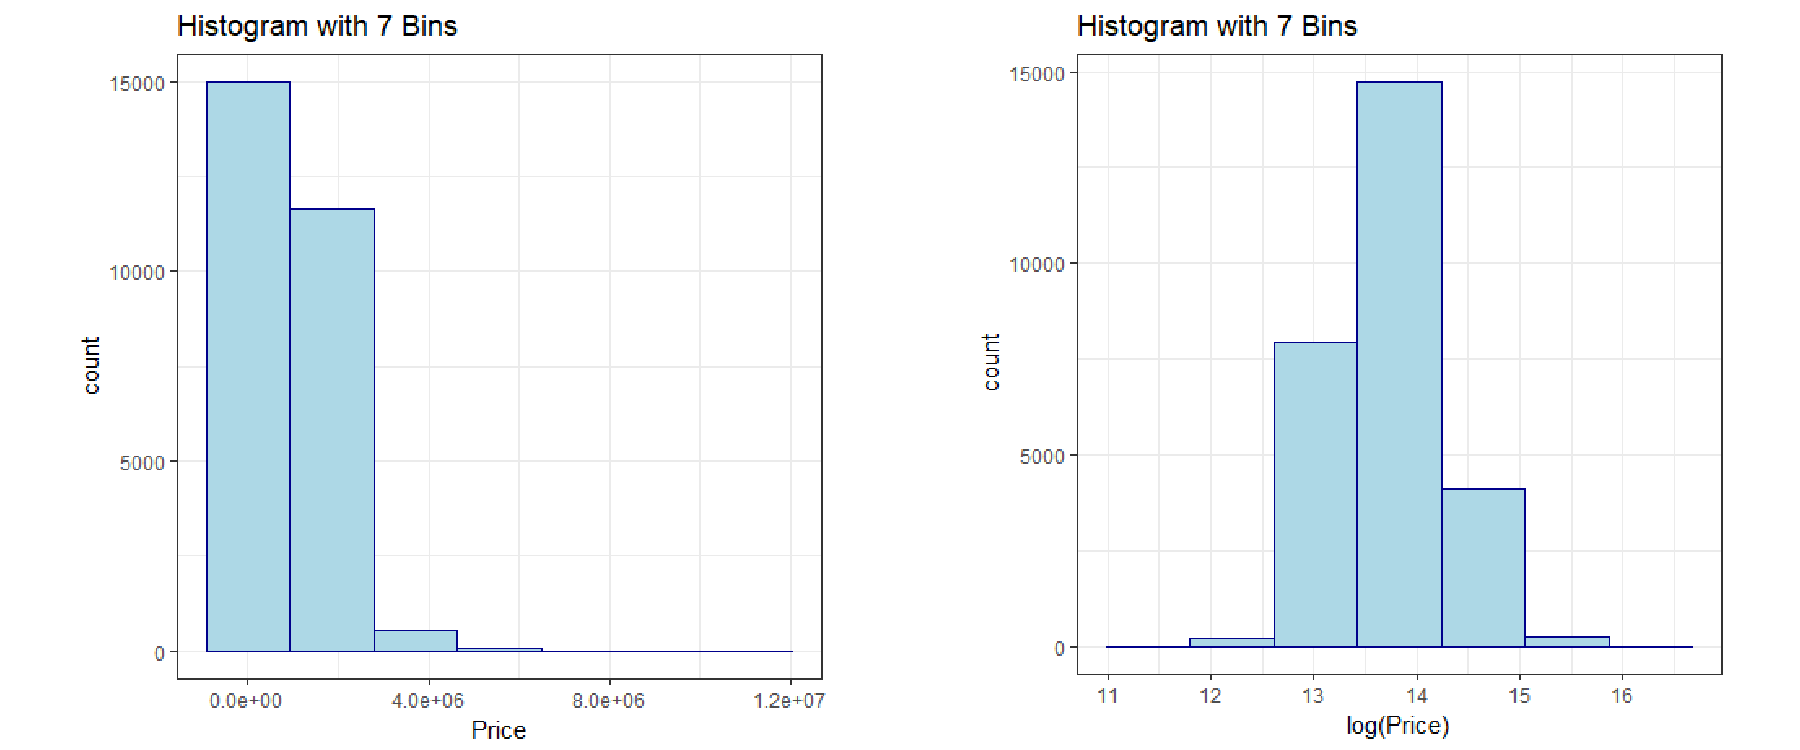
\includegraphics{Report_files/figure-latex/unnamed-chunk-7-1.pdf}
\caption{(a) Histogram of Price (b) Histogram of log(Price)}
\end{figure}

If we set the number of bins to 7 and plot a histogram of the Price
variable we find the distribution to be extremely skewed, and most of
the bins having very less observation. This is not a very representative
way of clustering the Price distribution. This is due to the presence of
certain outliers - the extremely high priced houses which are just a
handful but the majority belong to the lower range of Price therefore
this disparity.

To deal with this issue we apply a log tranformation on the Price and as
seen in the Figure 1(b) it comes in a normal shape dealing with the long
tailed distribution. So after analyzing multiple number of clusters we
have finally decided to stay with 7 clusters for our further analysis.

Next we set a new variable \emph{pricecluster} which has a value of 1 if
it is in the first bin, 2 if in the second bin and so on. This variable
represents our assumption of how houses are divided based on price.

\textbf{Rooms and Bathrooms:} I think these two features matter a lot in
determining the price of a property. So first we cluster based on these
two variables. But these two variables are \emph{Ordinal Variables}, so
we need to convert them into numerical to be used in k-means using the
following scheme:

If an ordinal variable has values \(i = 1,2,...,M\) then we convert them
using \[f(i) = \frac{i - 0.5}{M}\]

Next we fit a k-means clustering algorithm with 7 clusters and eucledian
distance.

\begin{figure}
\centering
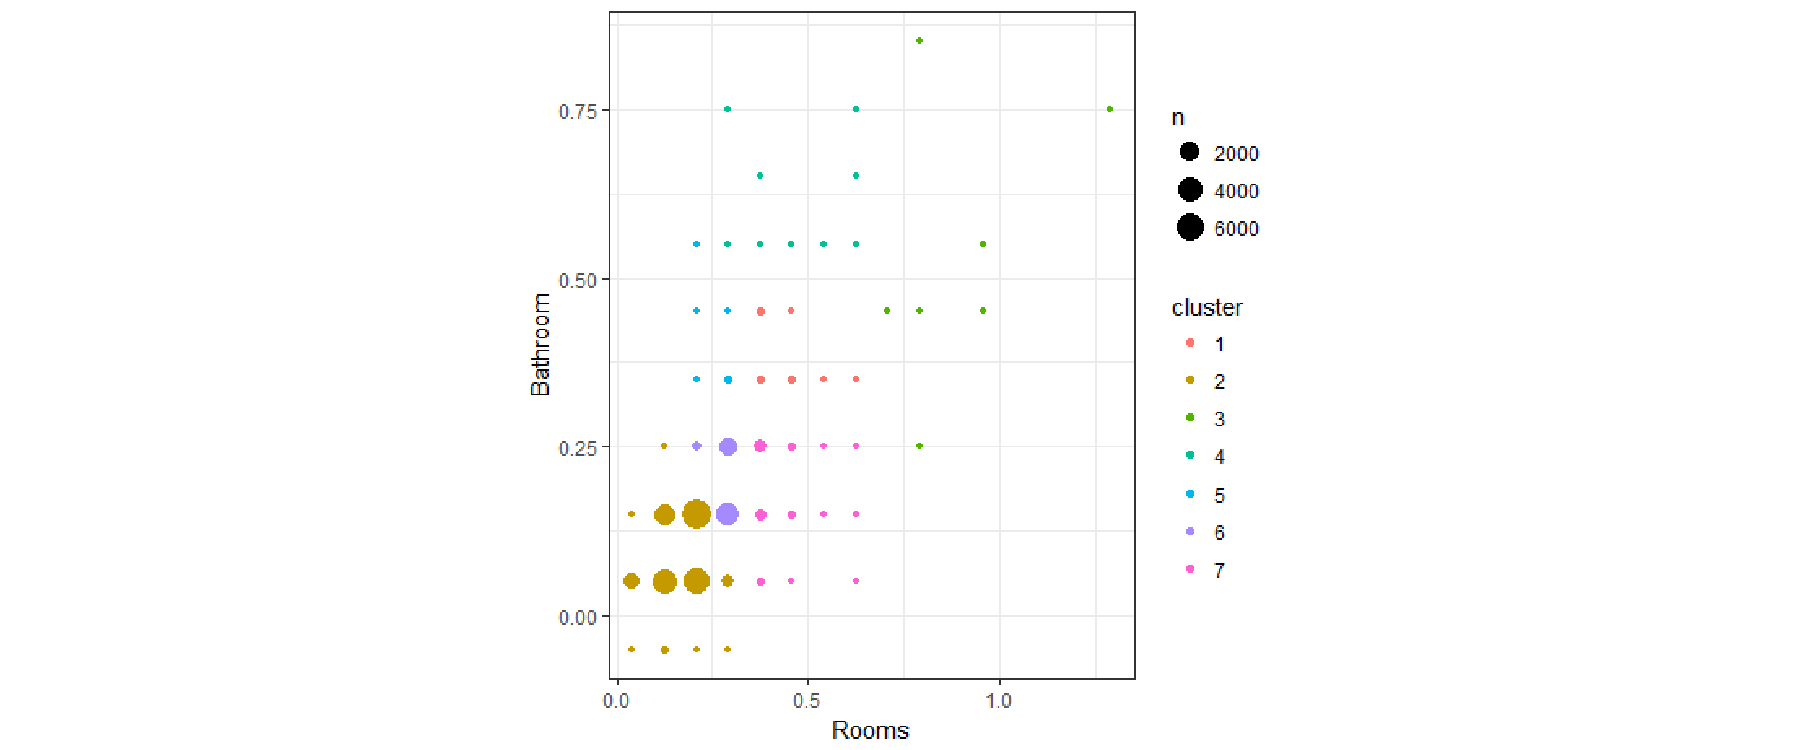
\includegraphics{Report_files/figure-latex/unnamed-chunk-8-1.pdf}
\caption{Clusters plotted with Bathroom and Rooms}
\end{figure}

The clusters are well defined with less bathrooms and rooms clustered
into one group and so on along the lines of the difference in number of
bathrooms and rooms the clusters are spread, and that makes quite some
sense when we predict price. As we have seen in Question 1 analysis that
less number of bathrooms and rooms are having less price while those
with more bathrooms and rooms are more pricey. But we had also seen some
patterns as some of the 1 BHK properties were high priced, those cannot
be understood by just bathrooms and rooms so we move with other
features.

Since these two are very well formed variables so as we had expected the
within cluster sum of squares is less.

\begin{longtable}[]{@{}ccccccc@{}}
\caption{within cluster sum of squares}\tabularnewline
\toprule
Clust 1 & Clust 2 & Clust 3 & Clust 4 & Clust 5 & Clust 6 & Clust
7\tabularnewline
\midrule
\endfirsthead
\toprule
Clust 1 & Clust 2 & Clust 3 & Clust 4 & Clust 5 & Clust 6 & Clust
7\tabularnewline
\midrule
\endhead
0.767 & 112.146 & 0.51 & 0.233 & 0.227 & 14.285 & 4.979\tabularnewline
\bottomrule
\end{longtable}

\textbf{Car}: Another important factor governing the price of a
property. But this again is an ordinal variable so we have to convert it
into a numerical variable using the above mentioned formula. We again
use 7 clusters with euclidean distance.

\begin{figure}
\centering
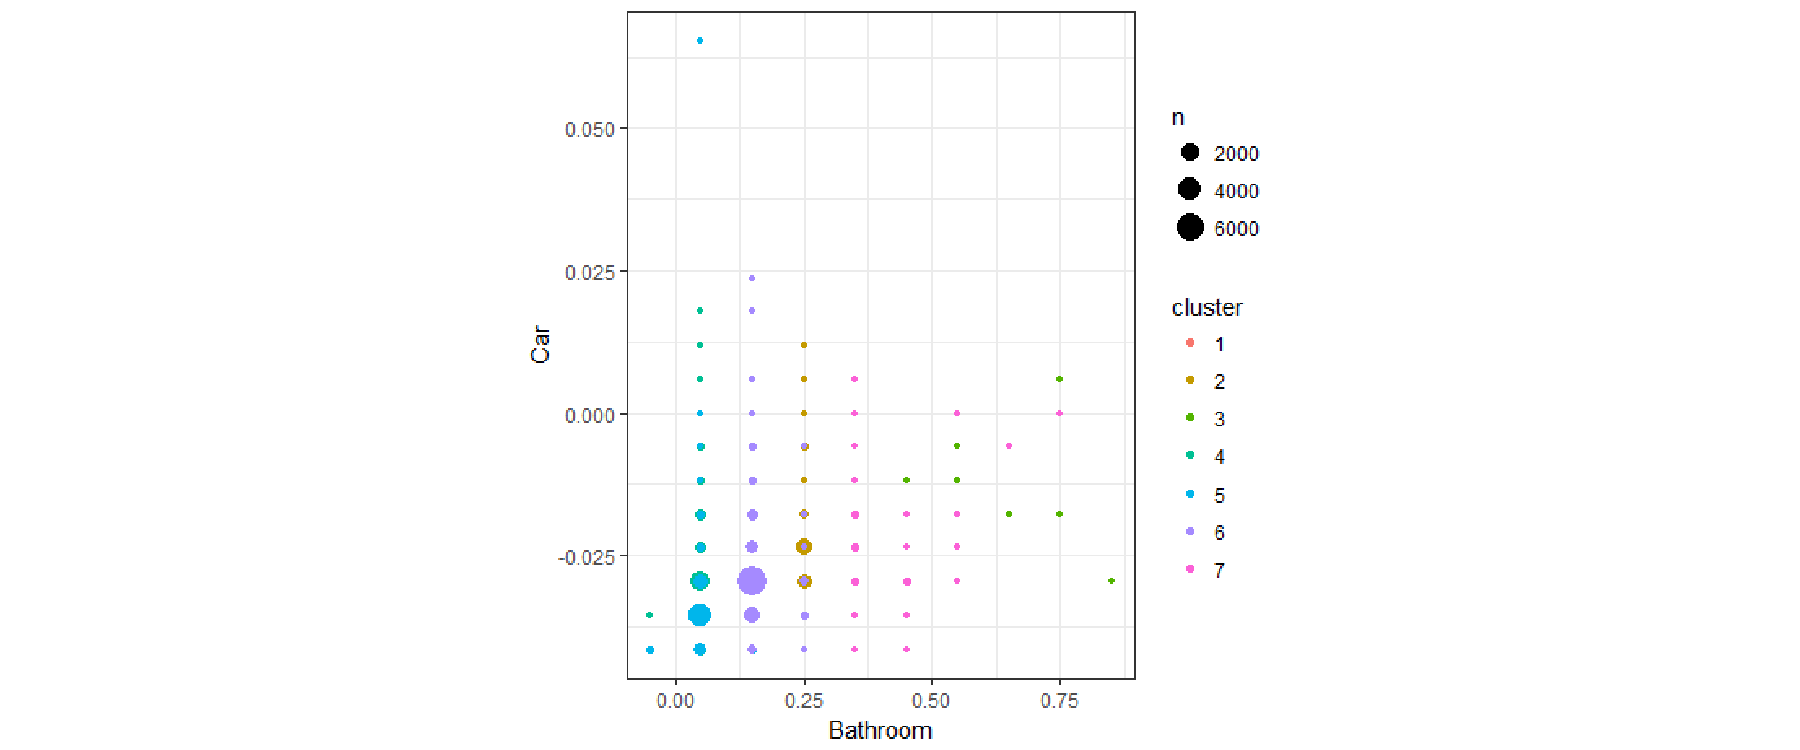
\includegraphics{Report_files/figure-latex/unnamed-chunk-10-1.pdf}
\caption{Clusters plotted with Bathroom and Car}
\end{figure}

From the plot we can see that Bathroom is a bigger factor in clustering
than Car. But also as the number of Bathrooms go high the Car variable
starts to make a difference. So we can conclude from this that as number
of bathrooms go higher after a point it does not make a difference with
the number of bathrooms but at that time the number of cars makes more
of an impact.

\begin{longtable}[]{@{}ccccccc@{}}
\caption{within cluster sum of squares}\tabularnewline
\toprule
Clust 1 & Clust 2 & Clust 3 & Clust 4 & Clust 5 & Clust 6 & Clust
7\tabularnewline
\midrule
\endfirsthead
\toprule
Clust 1 & Clust 2 & Clust 3 & Clust 4 & Clust 5 & Clust 6 & Clust
7\tabularnewline
\midrule
\endhead
1.894 & 3.418 & 1.92 & 4.591 & 25.712 & 18.096 & 1.493\tabularnewline
\bottomrule
\end{longtable}

From the above table we can see that the within cluster sum of squares
have reduced with Car variable.

\textbf{Distance}: Another very important feature is the Distance from
CBD which matters a lot when deciding the price of a property because
people like to stay close to city centers. Thus we include this also in
our clustering with K-means and 7 clusters.

\begin{figure}
\centering
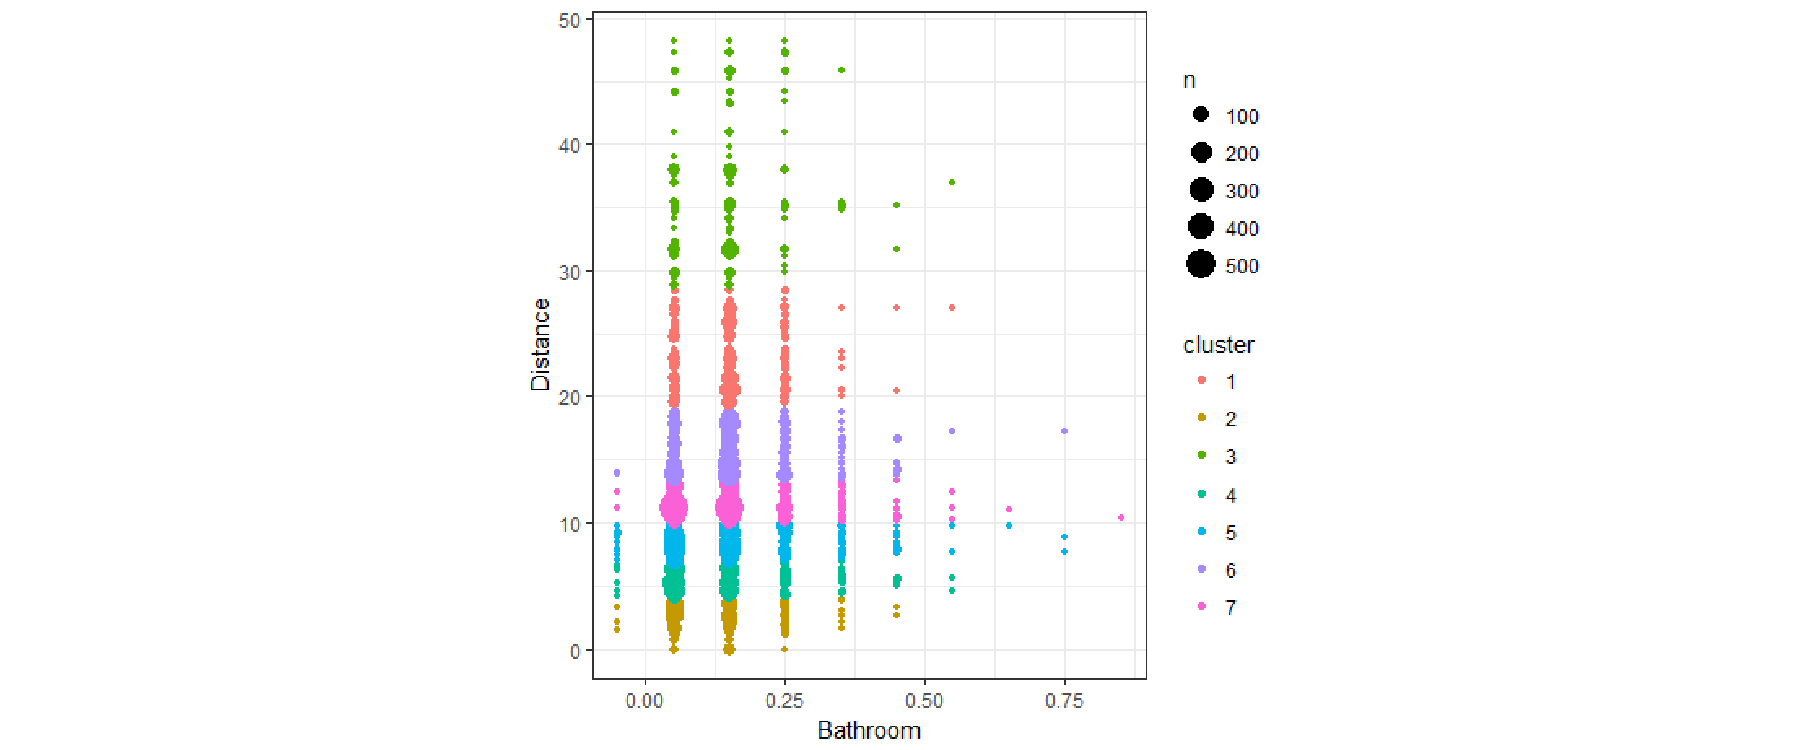
\includegraphics{Report_files/figure-latex/unnamed-chunk-12-1.pdf}
\caption{Clusters plotted with Bathroom and Distance}
\end{figure}

We see two very interesting things and would help us a lot in our
predictions. This time we get very clear clusters and we see that
Distance is such a strong variable in this clustering as we had
expected.

But at the same time from the table we see that the within cluster sum
of squares has gone very high. The reason? Distance was not normalized
while all the other variables lie between 0 and 1. So we have to
normalize our numerical variables before predicting.

\begin{longtable}[]{@{}ccccccc@{}}
\caption{within cluster sum of squares}\tabularnewline
\toprule
Clust 1 & Clust 2 & Clust 3 & Clust 4 & Clust 5 & Clust 6 & Clust
7\tabularnewline
\midrule
\endfirsthead
\toprule
Clust 1 & Clust 2 & Clust 3 & Clust 4 & Clust 5 & Clust 6 & Clust
7\tabularnewline
\midrule
\endhead
13279.76 & 2051.438 & 16554.62 & 2825.868 & 3611.635 & 13712.44 &
5270.14\tabularnewline
\bottomrule
\end{longtable}

\pagebreak

\section{3. Prediction Models for Predicting
Price}\label{prediction-models-for-predicting-price}

Before we begin our predictive modeling we had to do some preprocessing
steps.

\begin{itemize}
\tightlist
\item
  Firstly we normalized each of the numerical and integer variables to
  bring their values in between 0 and 1
\item
  We applied log transformation to Landsize since it had outliers and in
  Question 1 we decided to deal with this by taking a log
  transformation.
\item
  We selected ``Rooms'', ``Type'', ``Method'', ``Distance'',
  ``Bathroom'', ``Car'', ``Landsize'', ``Propertycount'',
  ``CouncilArea'' as our predictor variables.
\item
  Some of the categorical variables like ``Type'', ``Method'',
  ``CouncilArea'' was one hot encoded.
\end{itemize}

Next we randomly split the data into train-test split, 70\% data as
training data and remaining 30\% as testing.

\subsection{Penalized Regression
Models}\label{penalized-regression-models}

\textbf{Ridge Regression}

Ridge regression is the penalized version of linear regression where we
use \(L_2\) norm as the penalization term. The only tuning parameter
here is \(\lambda\) the regularization parameter.

The following plot shows the Mean Squared Error with different values of
lambda that we had tried.

\begin{figure}
\centering
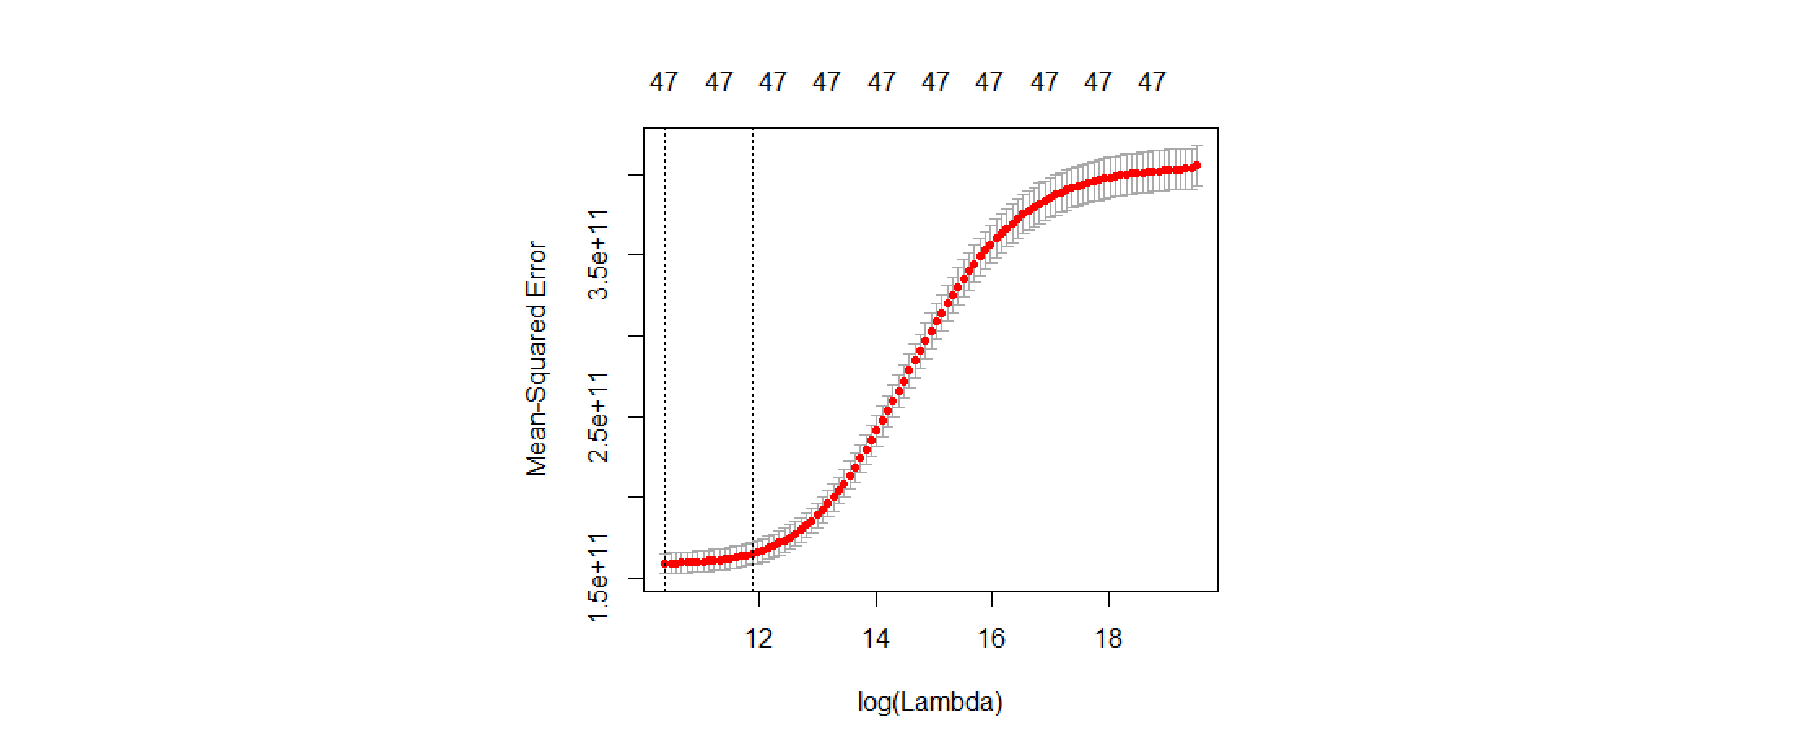
\includegraphics{Report_files/figure-latex/unnamed-chunk-14-1.pdf}
\caption{MSE with lambda values}
\end{figure}

The best performance is obtained at the following configuration:

\begin{longtable}[]{@{}ccc@{}}
\caption{Best performance lambda}\tabularnewline
\toprule
lambda & Training RMSE & Test RMSE\tabularnewline
\midrule
\endfirsthead
\toprule
lambda & Training RMSE & Test RMSE\tabularnewline
\midrule
\endhead
0.0295355 & 395895.2 & 407655.3\tabularnewline
\bottomrule
\end{longtable}

Following is the plot of the coefficients corresponding to each variable
that we used in the Ridge model. What we see is that \emph{Rooms,
Bathroom, Cars} have a positive impact on the Price while
\emph{Distance} has a huge negative impact on Price. This was expected
and corroborates our hypothesis we made in question 1.

\begin{figure}
\centering
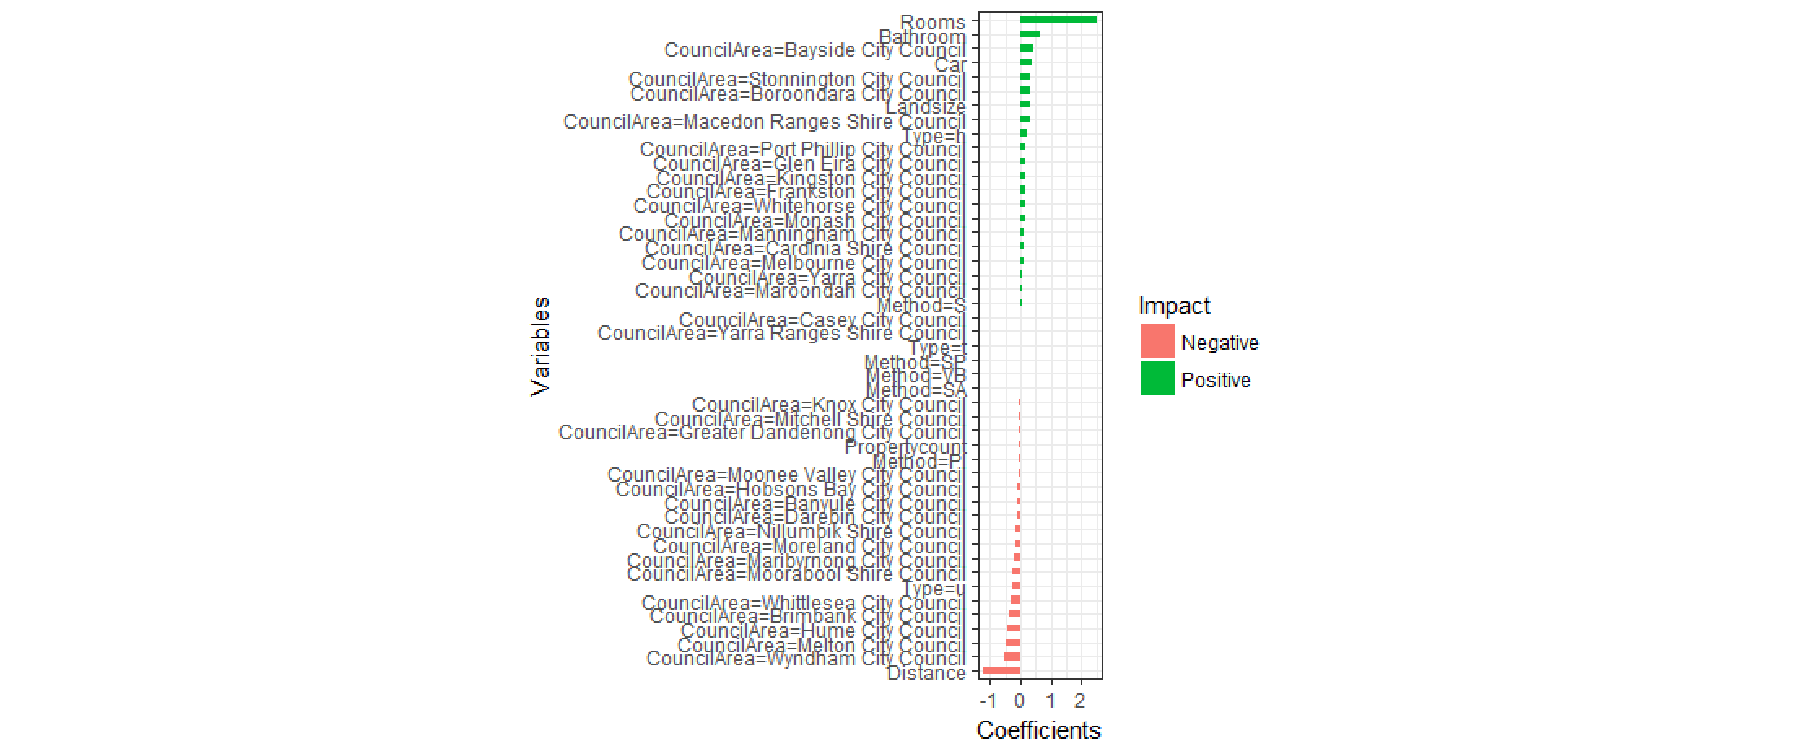
\includegraphics{Report_files/figure-latex/unnamed-chunk-16-1.pdf}
\caption{Variables and Coefficients}
\end{figure}

Since this is Ridge we do not see a lot of zero coefficients, but in
Lasso we might expect to see a lot more zero coefficients.

\textbf{Advantage and Disadvantages:} It has a regularization effect so
reduces overfitting. Computationally not expensive. Values of \(\beta\)
are small so it scales pretty well.

Cannot be used for reducing dimensions since it does not reduce any
coefficients to zero, as lasso does. Works well only if there is a
linear boundary/linear relationship between predictors and response. Not
very good with sparse features.

\textbf{Lasso Regression}

Lasso regression is the penalized version of linear regression where we
use \(L_1\) norm as the penalization term. The only tuning parameter
here is \(\lambda\) the regularization parameter. This is also used as
variable selection method many times since this algorithm sets
coefficients to zero if the importance of that variable is very low.

The following plot shows the Mean Squared Error with different values of
lambda that we had tried.

\begin{figure}
\centering
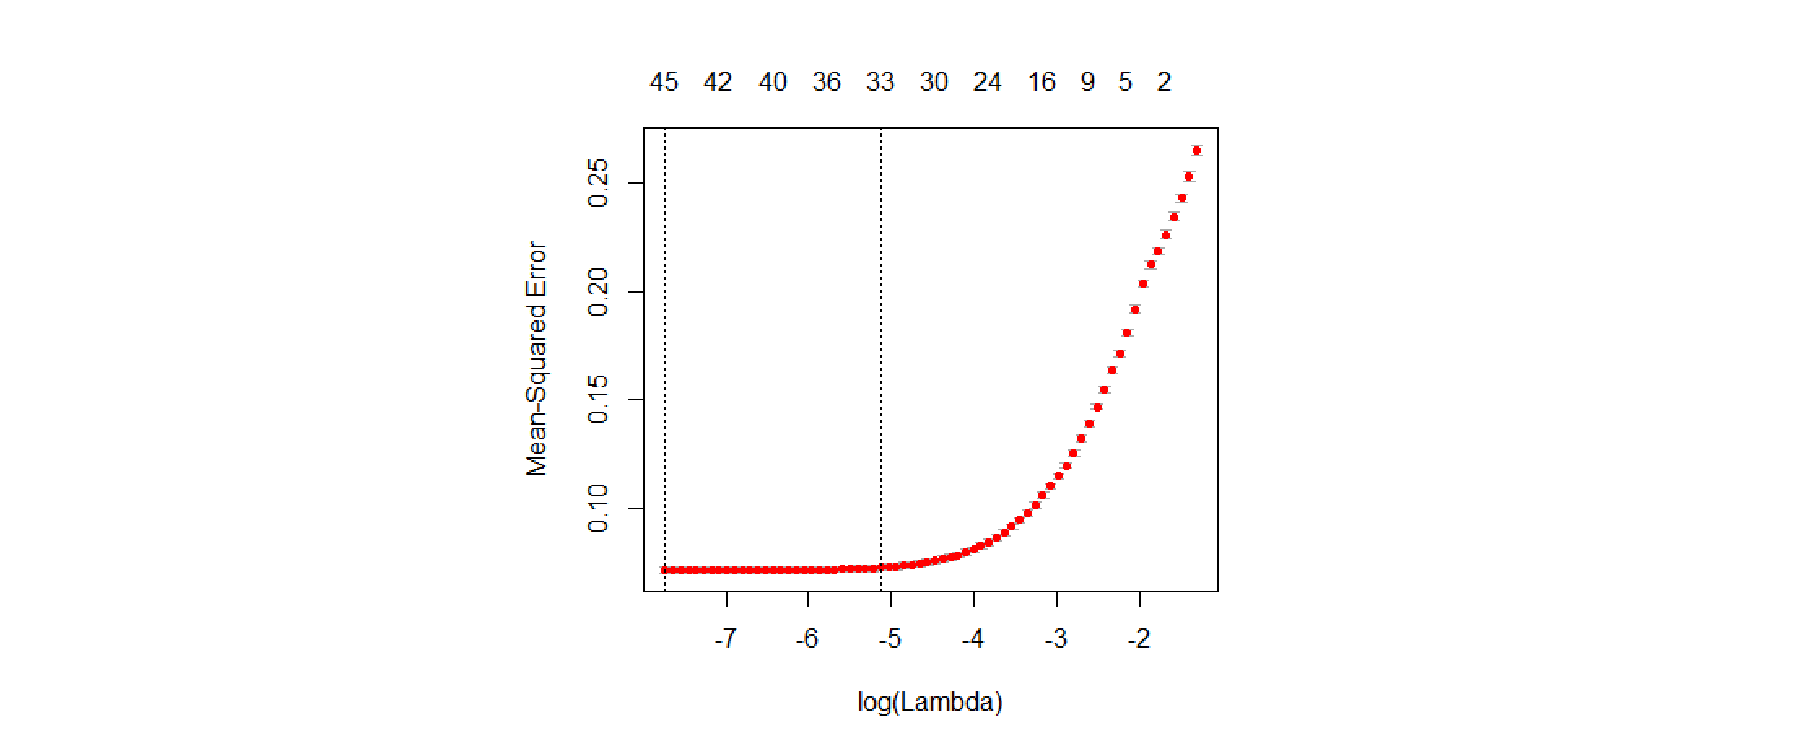
\includegraphics{Report_files/figure-latex/unnamed-chunk-17-1.pdf}
\caption{MSE with lambda values}
\end{figure}

The best performance is obtained at the following configuration:

\begin{longtable}[]{@{}ccc@{}}
\caption{Best performance lambda}\tabularnewline
\toprule
lambda & Training RMSE & Test RMSE\tabularnewline
\midrule
\endfirsthead
\toprule
lambda & Training RMSE & Test RMSE\tabularnewline
\midrule
\endhead
0.0004386 & 395302 & 402914.1\tabularnewline
\bottomrule
\end{longtable}

Following is the plot of the coefficients corresponding to each variable
that we used in the Ridge model. What we see is that \emph{Rooms,
Bathroom, Cars, certain CouncilArea} have a positive impact on the Price
while \emph{Distance} has a huge negative impact on Price. This was
expected and corroborates our hypothesis we made in question 1.

\begin{figure}
\centering
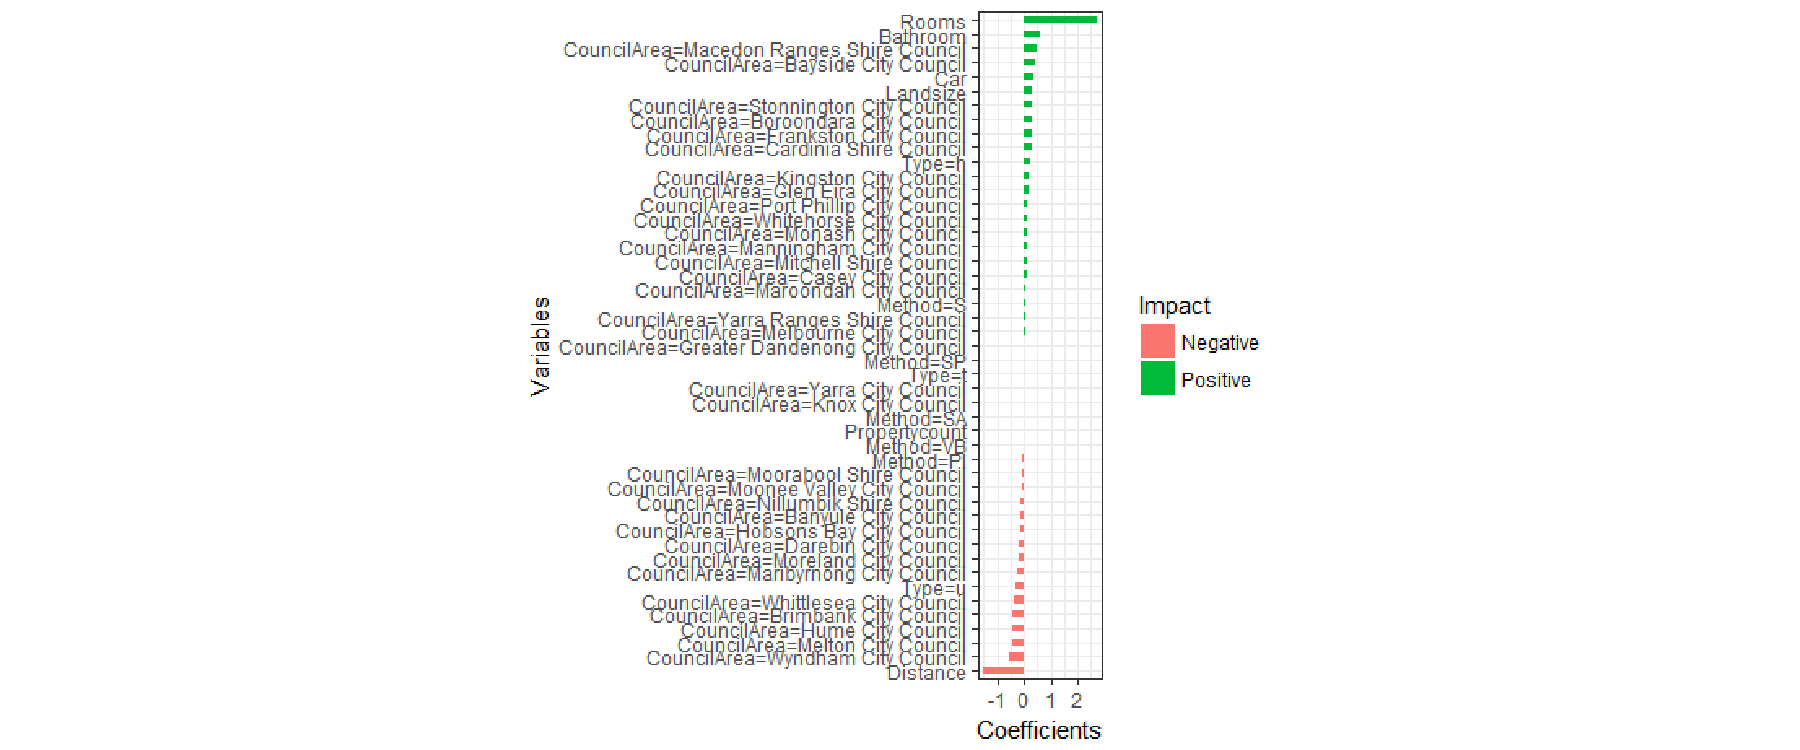
\includegraphics{Report_files/figure-latex/unnamed-chunk-19-1.pdf}
\caption{Variables and Coefficients}
\end{figure}

In Lasso we expect to see a lot of zero coefficients and here we see the
same from the above plot.

\textbf{Advantage and Disadvantages:} It has a regularization effect so
reduces overfitting. Computationally not expensive. Values of \(\beta\)
are small so it scales pretty well. Can be used for variable selection
as well.

Cannot deal with the situation where the number of predictors is greater
than number of samples. With correlated variables the behaviour is
eratic.

\subsection{Non Parametric Models}\label{non-parametric-models}

\textbf{K nearest neighbors} In K-nearest neighbor also known as knn
predicts the response variable by averaging over the values of the
response variables of the k nearest training examples. In this situation
it might work well because this is more driven by geography and nearest
neighbours makes more sense. Think of it in terms of neighborhood, in a
posh neighbourhood the costs are high whereas in locations not so posh
its low.

The only hyperparameter in this algorithm is the value of k, and since
we have already fixed the type of distance measure to eucledian so we
are only worried about trying different values of k.

We tried values k = (3, 9, 15, 21, 27) and here is the plot of
cross-validation RMSE with different values of k

\begin{figure}
\centering
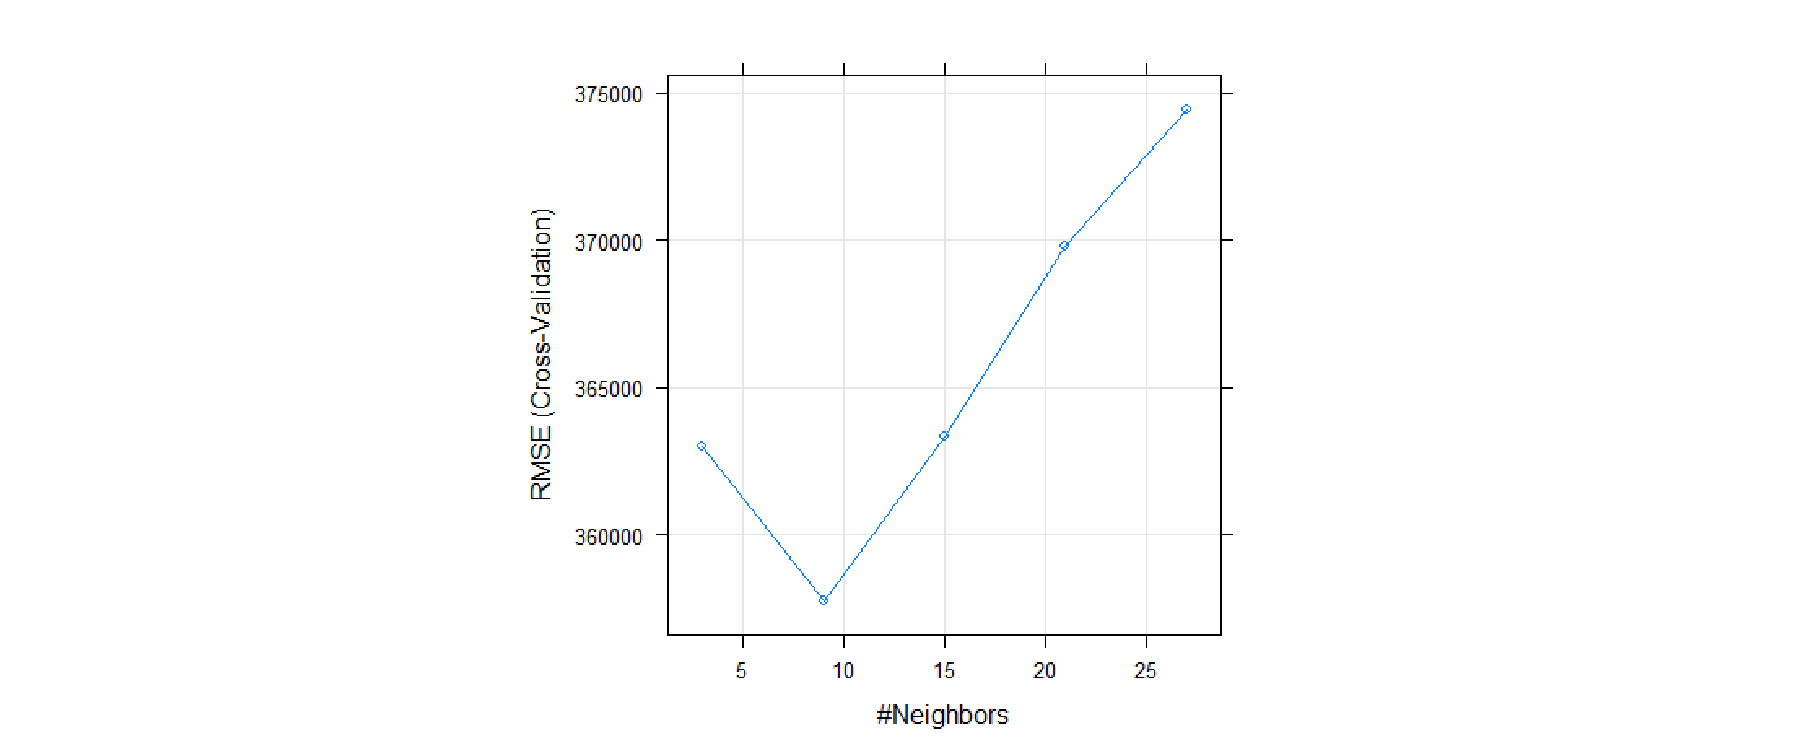
\includegraphics{Report_files/figure-latex/unnamed-chunk-20-1.pdf}
\caption{cross-validation RMSE with different values of k}
\end{figure}

The best results are got at k = 9

\begin{longtable}[]{@{}ccc@{}}
\caption{Best performance k in KNN}\tabularnewline
\toprule
k & Training RMSE & Test RMSE\tabularnewline
\midrule
\endfirsthead
\toprule
k & Training RMSE & Test RMSE\tabularnewline
\midrule
\endhead
9 & 357165.5 & 372030.7\tabularnewline
\bottomrule
\end{longtable}

KNN seems to give the best result out of the 4 algorithms. The residue
vs actual-value plot is as below and it shows that the residues are
closer to 0 as compared to gbm(in the next section)

\begin{figure}
\centering
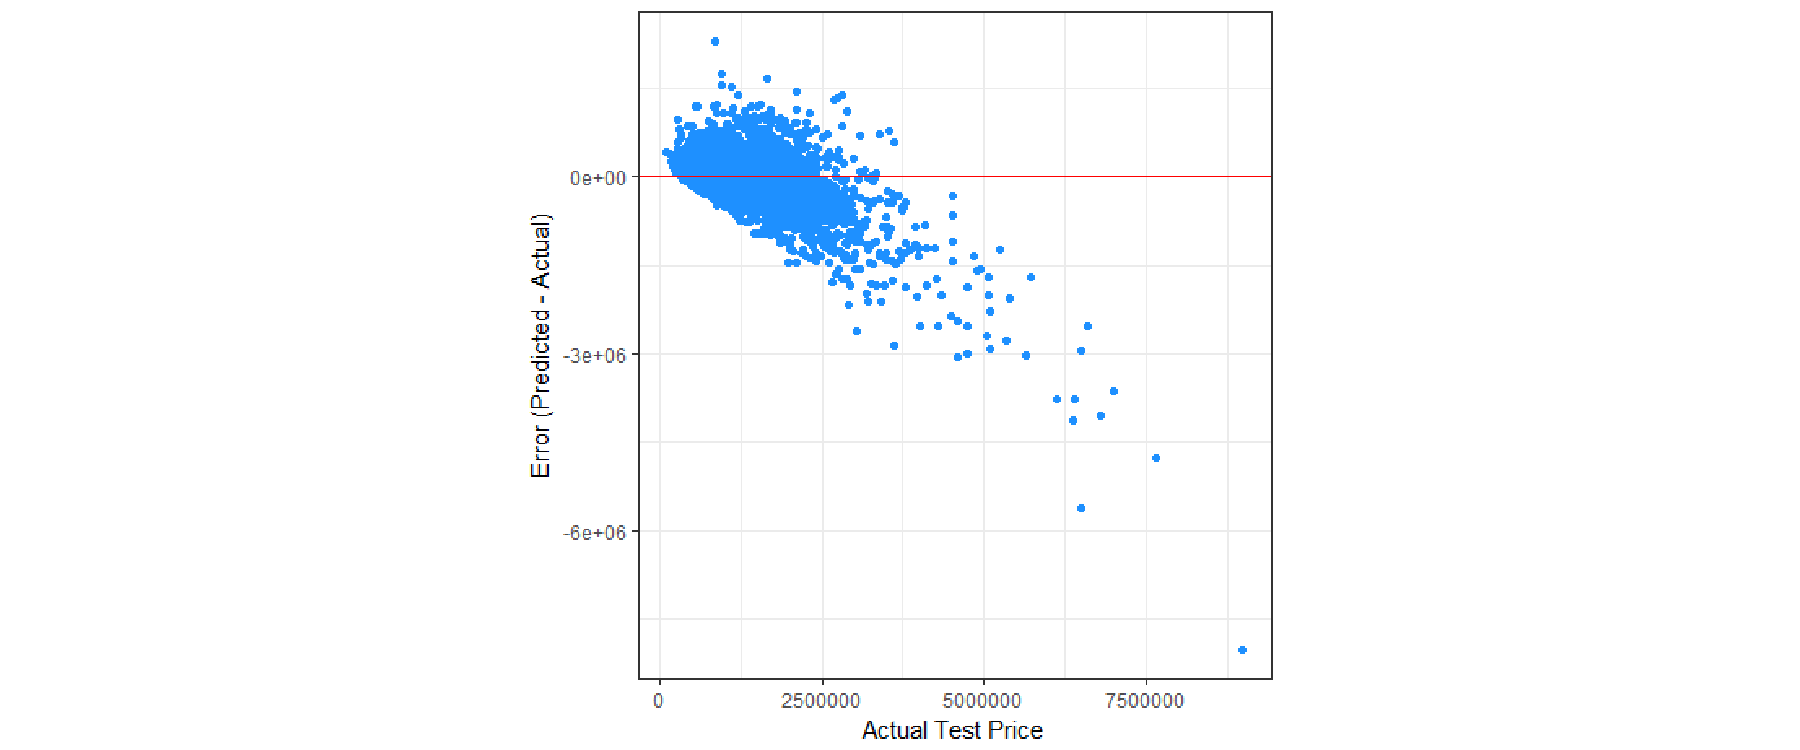
\includegraphics{Report_files/figure-latex/unnamed-chunk-22-1.pdf}
\caption{residue vs actual value}
\end{figure}

\textbf{Advantages and Disadvantages:} Robust to noisy data. Effective
in training large datasets, training time is very low.

Need to determine the value of k before starting. It is unclear what
distance measure to use in complicated features. Computation query is
quite high in test time.

\textbf{GBM: Generalized Boosted Regression Models} GBM is a boosting
algorithm, it creates an ensemble regressor, i.e.~you take many such
weak regressors, each slightly different, and then make a prediction
based on all of their predictions. The weights on each of these
regressors is computed based on how well it regresses a weighted
training set.

The hyperparameters that we have tuned are \emph{n.trees} - The number
of regressors/trees that are to be ensembled. The number of basis
functions in the additive expansion. \emph{interaction.depth} - The
maximum depth of variable interactions.

We took the following values of ``n.trees'' and ``interaction.depth''

\begin{Shaded}
\begin{Highlighting}[]
\NormalTok{ntrees =}\StringTok{ }\KeywordTok{c}\NormalTok{(}\DecValTok{1000}\NormalTok{, }\DecValTok{2000}\NormalTok{, }\DecValTok{2500}\NormalTok{)}
\NormalTok{interationdepth =}\StringTok{ }\KeywordTok{c}\NormalTok{(}\DecValTok{1}\NormalTok{, }\DecValTok{5}\NormalTok{, }\DecValTok{9}\NormalTok{)}
\end{Highlighting}
\end{Shaded}

The plot shows the test RMSE for each configuration:

\begin{figure}
\centering
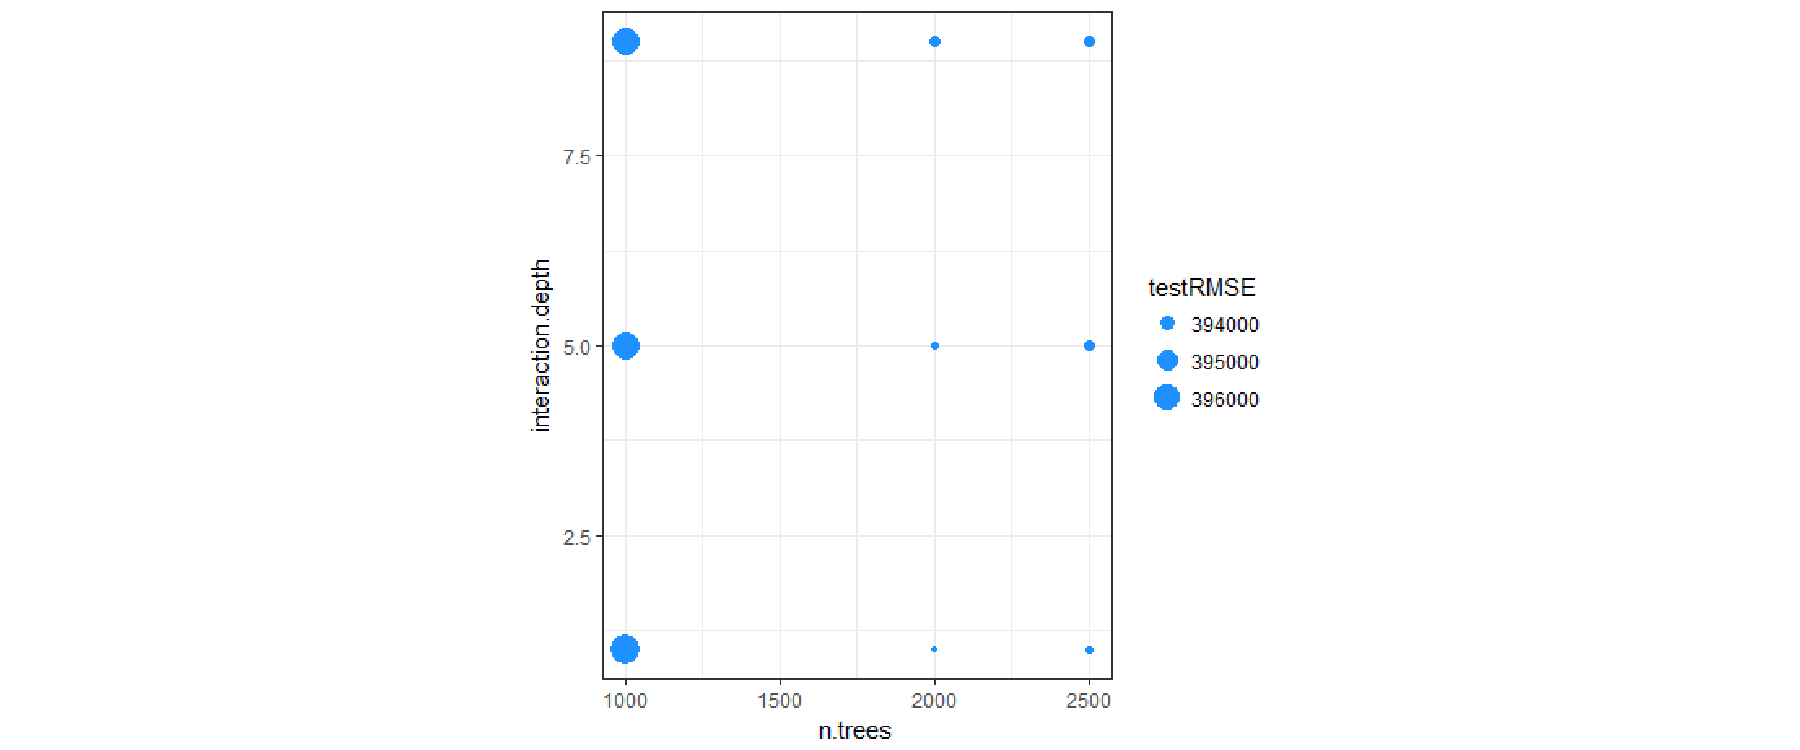
\includegraphics{Report_files/figure-latex/unnamed-chunk-24-1.pdf}
\caption{RMSE for different configurations of hyperparameters}
\end{figure}

The best results are got at n.trees = 2000 and interaction.depth = 1

\begin{longtable}[]{@{}cccc@{}}
\caption{Best performance in GBM}\tabularnewline
\toprule
n.trees & interaction.depth & Training RMSE & Test RMSE\tabularnewline
\midrule
\endfirsthead
\toprule
n.trees & interaction.depth & Training RMSE & Test RMSE\tabularnewline
\midrule
\endhead
2000 & 1 & 386418.8 & 393516.6\tabularnewline
\bottomrule
\end{longtable}

We can have a look at the The residue vs actual-value plot, we can see
that the plot is not as good as that of KNN and the residuals are not
equally distributed around the 0 mark.

\begin{figure}
\centering
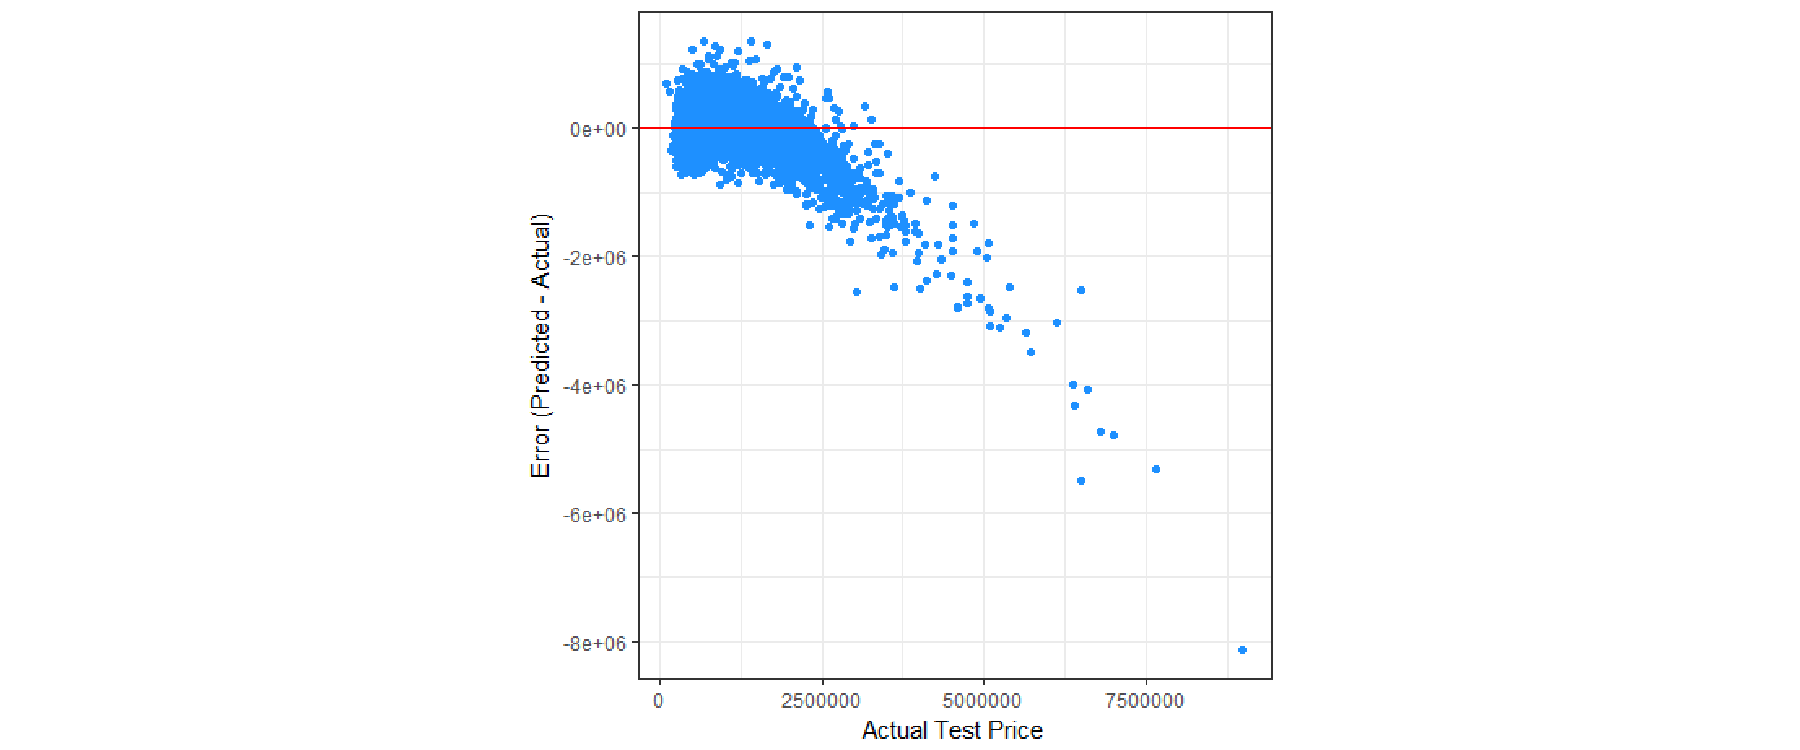
\includegraphics{Report_files/figure-latex/unnamed-chunk-26-1.pdf}
\caption{Residue vs Actual value}
\end{figure}

GBM also gives us information about the variable importance that we can
see in the below plot.

\begin{figure}
\centering
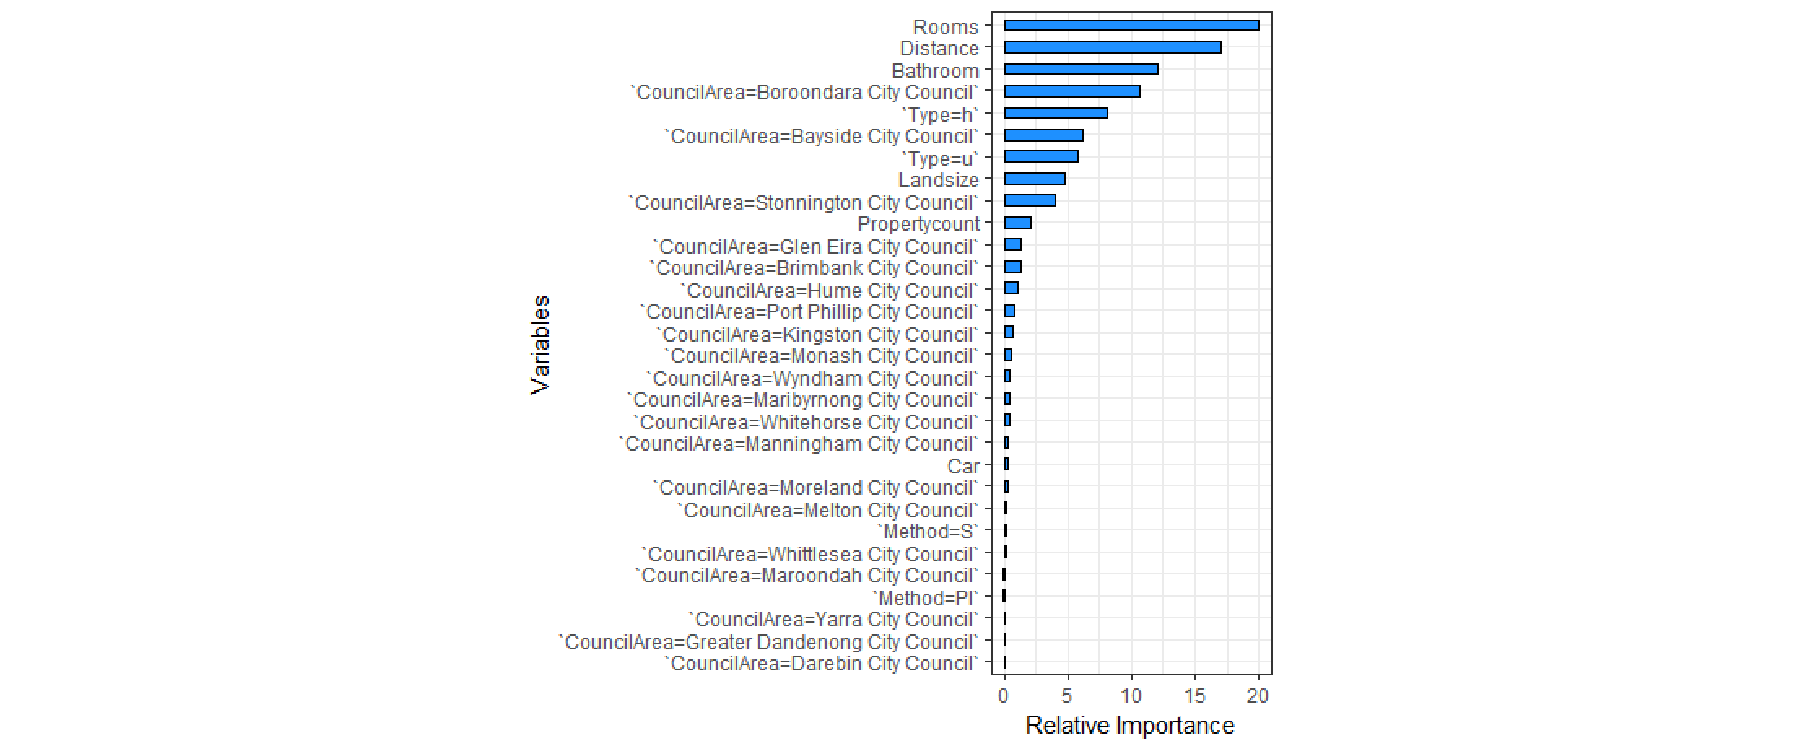
\includegraphics{Report_files/figure-latex/unnamed-chunk-27-1.pdf}
\caption{Variable Importance in GBM}
\end{figure}

\textbf{Advantages and Disadvantages} Boosting based methods generally
give better results but they are harder to fit than Random Forests. It
manages the missing values by itself. Can handle categorical data
easily.

GBM training generally takes longer because of the fact that trees are
built sequentially. Requires a lot of memory since we have to store all
the trees in memory.

\pagebreak

\section{4. A new approach to improve
performance}\label{a-new-approach-to-improve-performance}

An approach which I think will improve performance is \textbf{stacking
the models} together.

Stacking (also called meta ensembling) is a model ensembling technique
used to combine information from multiple predictive models to generate
a new model. Often times the stacked model (also called 2nd-level model)
will outperform each of the individual models due its smoothing nature
and ability to highlight each base model where it performs best and
discredit each base model where it performs poorly. For this reason,
stacking is most effective when the base models are significantly
different.

\textbf{Intuition:} Think of stacking as basically an exploitation of
the central limit theorem.

The central limit theorem loosely says that, as the sample size
increases, the mean of the sample will become an increasingly accurate
estimate of the actual location of the population mean (assuming that's
the statistic you're looking at), and the variance will tighten.

If you have one model and it produces one prediction for your dependent
variable, that prediction will likely be high or low to some degree. But
if you have 3 or 5 or 10 different models that produce different
predictions, for any given observation, the high predictions from some
models will tend to offset the low errors from some other models, and
the net effect will be a convergence of the average (or other
combination) of the predictions towards ``the truth.'' Not on every
observation, but in general that's the tendency. And so, generally, an
stacked model will outperform the best single model.

\textbf{Computational Challenges:} Our approach is simple so we did not
face much of a computational challenge. We take the predictions from all
the four predictive models in question 3 and give weights to the outputs
from the models. For us KNN performed the best followed by GBM, then
Lasso and worst performance was seen in Ridge.

Therefore we multiply 0.4 to predictions of KNN, 0.3 to predictions of
GBM, 0.2 to predictions of Lasso and 0.1 to predictions of Ridge. We
must be careful that the sum of the weights need to add upto 1 otherwise
the weights would not make sense.

\begin{Shaded}
\begin{Highlighting}[]
\StringTok{'''}
\StringTok{test_pred_gbm = GBM Prediction}
\StringTok{test_pred_knn = KNN prediction}
\StringTok{test_pred_lasso = Lasso Prediction}
\StringTok{test_pred_ridge = Ridge Prediction}
\StringTok{test_pred_stack = Stacked Prediction}
\StringTok{'''}

\NormalTok{test_pred_stack =}\StringTok{ }\NormalTok{(}\FloatTok{0.3}\OperatorTok{*}\NormalTok{test_pred_gbm }\OperatorTok{+}\StringTok{ }\FloatTok{0.4}\OperatorTok{*}\NormalTok{test_pred_knn }\OperatorTok{+}\StringTok{ }
\StringTok{                     }\FloatTok{0.2}\OperatorTok{*}\NormalTok{test_pred_lasso }\OperatorTok{+}\StringTok{ }\FloatTok{0.1}\OperatorTok{*}\NormalTok{test_pred_ridge)}
\end{Highlighting}
\end{Shaded}

\textbf{Results:} Stacking as expected outperformed all the algorithms
we had used in Question 3. The results are summarised in the following
table.

\begin{longtable}[]{@{}cc@{}}
\caption{Test RMSE for each approach}\tabularnewline
\toprule
Approach & Test RMSE\tabularnewline
\midrule
\endfirsthead
\toprule
Approach & Test RMSE\tabularnewline
\midrule
\endhead
Ridge & 407655.3\tabularnewline
Lasso & 402914.1\tabularnewline
KNN & 372030.7\tabularnewline
GBM & 393516.6\tabularnewline
Stacking & 363988.7\tabularnewline
\bottomrule
\end{longtable}


\end{document}
